% Options for packages loaded elsewhere
% Options for packages loaded elsewhere
\PassOptionsToPackage{unicode}{hyperref}
\PassOptionsToPackage{hyphens}{url}
\PassOptionsToPackage{dvipsnames,svgnames,x11names}{xcolor}
%
\documentclass[
  letterpaper,
  DIV=11,
  numbers=noendperiod]{scrartcl}
\usepackage{xcolor}
\usepackage{amsmath,amssymb}
\setcounter{secnumdepth}{-\maxdimen} % remove section numbering
\usepackage{iftex}
\ifPDFTeX
  \usepackage[T1]{fontenc}
  \usepackage[utf8]{inputenc}
  \usepackage{textcomp} % provide euro and other symbols
\else % if luatex or xetex
  \usepackage{unicode-math} % this also loads fontspec
  \defaultfontfeatures{Scale=MatchLowercase}
  \defaultfontfeatures[\rmfamily]{Ligatures=TeX,Scale=1}
\fi
\usepackage{lmodern}
\ifPDFTeX\else
  % xetex/luatex font selection
\fi
% Use upquote if available, for straight quotes in verbatim environments
\IfFileExists{upquote.sty}{\usepackage{upquote}}{}
\IfFileExists{microtype.sty}{% use microtype if available
  \usepackage[]{microtype}
  \UseMicrotypeSet[protrusion]{basicmath} % disable protrusion for tt fonts
}{}
\makeatletter
\@ifundefined{KOMAClassName}{% if non-KOMA class
  \IfFileExists{parskip.sty}{%
    \usepackage{parskip}
  }{% else
    \setlength{\parindent}{0pt}
    \setlength{\parskip}{6pt plus 2pt minus 1pt}}
}{% if KOMA class
  \KOMAoptions{parskip=half}}
\makeatother
% Make \paragraph and \subparagraph free-standing
\makeatletter
\ifx\paragraph\undefined\else
  \let\oldparagraph\paragraph
  \renewcommand{\paragraph}{
    \@ifstar
      \xxxParagraphStar
      \xxxParagraphNoStar
  }
  \newcommand{\xxxParagraphStar}[1]{\oldparagraph*{#1}\mbox{}}
  \newcommand{\xxxParagraphNoStar}[1]{\oldparagraph{#1}\mbox{}}
\fi
\ifx\subparagraph\undefined\else
  \let\oldsubparagraph\subparagraph
  \renewcommand{\subparagraph}{
    \@ifstar
      \xxxSubParagraphStar
      \xxxSubParagraphNoStar
  }
  \newcommand{\xxxSubParagraphStar}[1]{\oldsubparagraph*{#1}\mbox{}}
  \newcommand{\xxxSubParagraphNoStar}[1]{\oldsubparagraph{#1}\mbox{}}
\fi
\makeatother


\usepackage{longtable,booktabs,array}
\usepackage{calc} % for calculating minipage widths
% Correct order of tables after \paragraph or \subparagraph
\usepackage{etoolbox}
\makeatletter
\patchcmd\longtable{\par}{\if@noskipsec\mbox{}\fi\par}{}{}
\makeatother
% Allow footnotes in longtable head/foot
\IfFileExists{footnotehyper.sty}{\usepackage{footnotehyper}}{\usepackage{footnote}}
\makesavenoteenv{longtable}
\usepackage{graphicx}
\makeatletter
\newsavebox\pandoc@box
\newcommand*\pandocbounded[1]{% scales image to fit in text height/width
  \sbox\pandoc@box{#1}%
  \Gscale@div\@tempa{\textheight}{\dimexpr\ht\pandoc@box+\dp\pandoc@box\relax}%
  \Gscale@div\@tempb{\linewidth}{\wd\pandoc@box}%
  \ifdim\@tempb\p@<\@tempa\p@\let\@tempa\@tempb\fi% select the smaller of both
  \ifdim\@tempa\p@<\p@\scalebox{\@tempa}{\usebox\pandoc@box}%
  \else\usebox{\pandoc@box}%
  \fi%
}
% Set default figure placement to htbp
\def\fps@figure{htbp}
\makeatother





\setlength{\emergencystretch}{3em} % prevent overfull lines

\providecommand{\tightlist}{%
  \setlength{\itemsep}{0pt}\setlength{\parskip}{0pt}}



 


\usepackage{sectsty}
\usepackage{xcolor}
\definecolor{primaryorange}{HTML}{E06E53}
\definecolor{secondaryorange}{HTML}{B8573E}
\sectionfont{\color{primaryorange}\sffamily}
\subsectionfont{\color{secondaryorange}\sffamily}
\subsubsectionfont{\color{secondaryorange}\sffamily}
\let\maketitle\relax
\KOMAoption{captions}{tableheading}
\makeatletter
\@ifpackageloaded{caption}{}{\usepackage{caption}}
\AtBeginDocument{%
\ifdefined\contentsname
  \renewcommand*\contentsname{Table of contents}
\else
  \newcommand\contentsname{Table of contents}
\fi
\ifdefined\listfigurename
  \renewcommand*\listfigurename{List of Figures}
\else
  \newcommand\listfigurename{List of Figures}
\fi
\ifdefined\listtablename
  \renewcommand*\listtablename{List of Tables}
\else
  \newcommand\listtablename{List of Tables}
\fi
\ifdefined\figurename
  \renewcommand*\figurename{Figure}
\else
  \newcommand\figurename{Figure}
\fi
\ifdefined\tablename
  \renewcommand*\tablename{Table}
\else
  \newcommand\tablename{Table}
\fi
}
\@ifpackageloaded{float}{}{\usepackage{float}}
\floatstyle{ruled}
\@ifundefined{c@chapter}{\newfloat{codelisting}{h}{lop}}{\newfloat{codelisting}{h}{lop}[chapter]}
\floatname{codelisting}{Listing}
\newcommand*\listoflistings{\listof{codelisting}{List of Listings}}
\makeatother
\makeatletter
\makeatother
\makeatletter
\@ifpackageloaded{caption}{}{\usepackage{caption}}
\@ifpackageloaded{subcaption}{}{\usepackage{subcaption}}
\makeatother
\usepackage{bookmark}
\IfFileExists{xurl.sty}{\usepackage{xurl}}{} % add URL line breaks if available
\urlstyle{same}
\hypersetup{
  pdftitle={ECOFLOR 2026: Book of Abstracts},
  colorlinks=true,
  linkcolor={primaryorange},
  filecolor={primaryorange},
  citecolor={primaryorange},
  urlcolor={primaryorange},
  pdfcreator={LaTeX via pandoc}}


\title{ECOFLOR 2026: Book of Abstracts}
\author{}
\date{}
\begin{document}
\maketitle


\begin{titlepage}
\centering
\vspace*{2cm}
{\Huge \textbf{ECOFLOR 2026: Book of Abstracts} \par}
\vspace{1.5cm}
\includegraphics[width=0.5\textwidth]{images/logo_without_bakground_small.png}
\vfill
{\Large \today \par}
\end{titlepage}

\newpage
\tableofcontents
\newpage

The ECOFLOR 2026 Book of Abstracts. The book may be downloaded as a PDF
file from the \href{https://ecoflor2026.com/}{ECOFLOR 2026 website}.

\section{Scientific Committee}\label{scientific-committee}

The 23rd edition of EcoFlor meeting was organised by \textbf{the
Wildlife Pollinators Group}, a research group of the
\href{https://weh.cat/}{\textbf{Wildlife Ecology and Health}
\textbf{Lab}}, based in the
\href{https://www.uab.cat/web/studies/graduate/university-master-s-degrees/by-areas-of-knowledge/veterinary-medicine-1345670299644.html}{Veterinary
Faculty of the Autonomous University of Barcelona (UAB).} Additional
researchers from different institutions (IRTA, CTFC, IVIA, CREAF) are
actively involved in the organisation.

In the Wildlife Pollinators Group we study the relationship between
large herbivores (domestic and wild) and plant-pollinator communities
and interactions,as well as in pollination function. We are also
interested in understanding how other processes operating at large
scales (such as wildfires) influence the assemblage of these
communities. On the opposite (microscopic scale) side, we are interested
in disentangling the mysteries behind solitary bee health. We conduct
basic faunistic studies as well as research on bee diversity patterns in
multiple types of habitats (including urban ecosystems, riparian
ecosystems, and grasslands).

\textbf{Organisation committee}: Carlos Hernández-Castellano, Néstor
Pérez-Méndez, Jordi Margalef-Marrassé, Alice Casiraghi, Jakub Štenc,
Júlia Batlle-Benaiges, Júlia Coromina, Nil Guerrero, Marina Aguilar
Grau,

\href{https://weh.cat/}{\begin{center}
\includegraphics[width=3.125in,height=\textheight,keepaspectratio]{images/wildlifelab.png}
\end{center}
}

\begin{minipage}[t]{0.45\textwidth}
\centering
\includegraphics[width=3.5cm]{images/people/CarlosHC.png}

\vspace{1em}
\textbf{Carlos Hernández-Castellano}

\href{mailto:carlos.hernandezcastellano@gmail.com}{✉️} \href{https://scholar.google.es/citations?user=N20Q75MAAAAJ\&hl=es}{\includegraphics[width=20pt]{images/scholar.png}}
\end{minipage}
\hfill
\begin{minipage}[t]{0.45\textwidth}
\centering
\includegraphics[width=3.5cm]{images/people/NestorPM.png}

\vspace{1em}
\textbf{Néstor Pérez-Méndez}

\href{mailto:nestor.perez@irta.cat}{✉️} \href{https://scholar.google.es/citations?user=9cVCRHcAAAAJ\&hl=es}{\includegraphics[width=20pt]{images/scholar.png}}
\end{minipage}

\vspace{2em}

\begin{minipage}[t]{0.45\textwidth}
\centering
\includegraphics[width=3.5cm]{images/people/AliceC.png}

\vspace{1em}
\textbf{Alice Casiraghi}

\href{mailto:theaphidologist@gmail.com}{✉️} \href{https://scholar.google.com/citations?user=J6BL1f0AAAAJ\&hl=es}{\includegraphics[width=20pt]{images/scholar.png}}
\end{minipage}
\hfill
\begin{minipage}[t]{0.45\textwidth}
\centering

\includegraphics[width=3.5cm]{images/people/jordi_real.png}

\vspace{1em}
\textbf{Jordi Margalef-Marrassé}

\href{mailto:jordi.margalef@ctfc.cat}{✉️} \href{https://scholar.google.com/citations?user=Os21VVYAAAAJ\&hl=ca}{\includegraphics[width=20pt]{images/scholar.png}}
\end{minipage}

\vspace{2em}

\begin{minipage}[t]{0.45\textwidth}
\centering
\includegraphics[width=3.5cm]{images/people/js3.png}

\vspace{1em}
\textbf{Jakub Štenc}

\href{mailto:jakubstenc@gmail.com}{✉️} \href{https://scholar.google.com/citations?user=QrFO4O0AAAAJ\&hl=cs}{\includegraphics[width=20pt]{images/scholar.png}} \href{https://jakubstenc.github.io/jakubstenc/CV.html}{CV}
\end{minipage}
\hfill
\begin{minipage}[t]{0.45\textwidth}
\centering
\includegraphics[width=3.5cm]{images/people/JuliaBB.png}

\vspace{1em}
\textbf{Júlia Batlle-Benaiges}

\href{mailto:ju.ba.benaiges@gmail.com}{✉️} \href{https://scholar.google.com/citations?user=cr9FBjkAAAAJ\&hl=ca}{\includegraphics[width=20pt]{images/scholar.png}}
\end{minipage}

\vspace{2em}

\begin{minipage}[t]{0.45\textwidth}
\centering
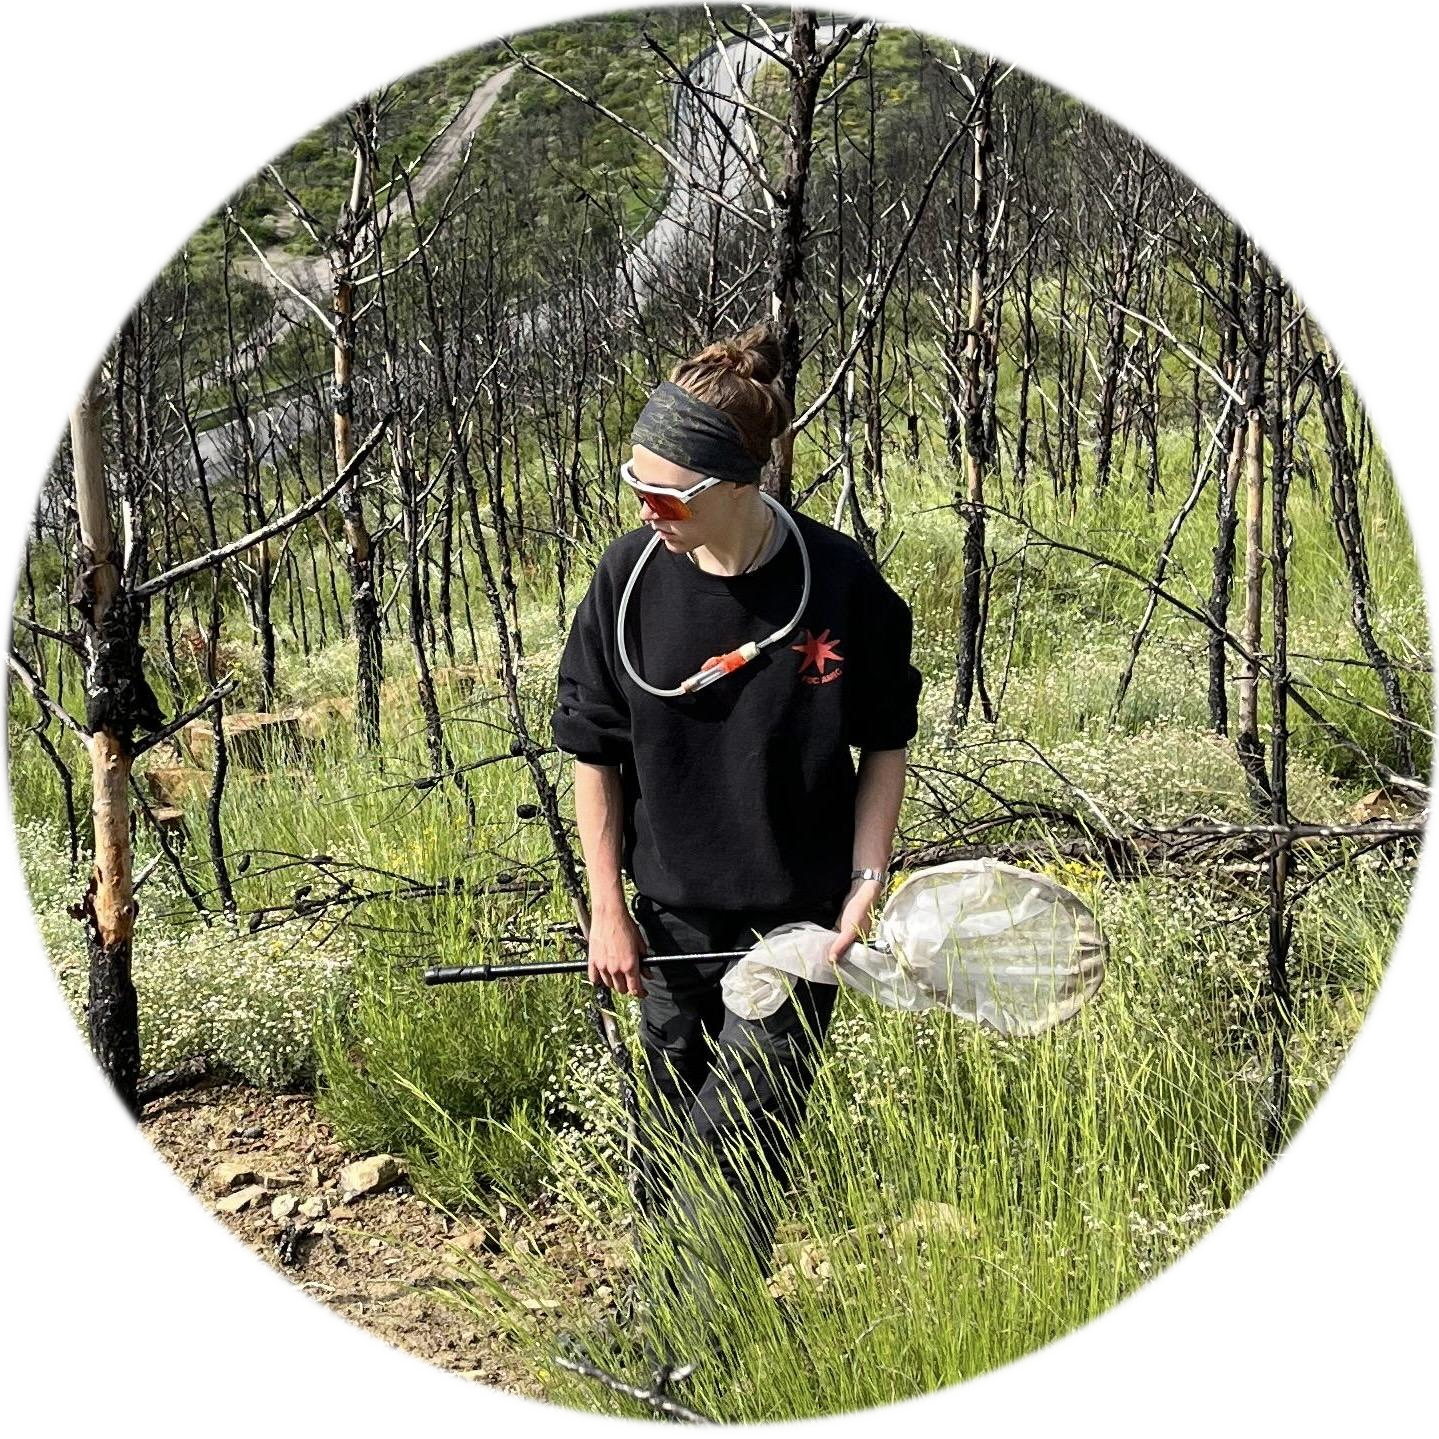
\includegraphics[width=3.5cm]{images/people/juliacoronira.png}

\vspace{1em}
\textbf{Júlia Coromina}

\href{mailto:jucoromina8@gmail.com}{✉️} \href{https://www.linkedin.com/in/j\%C3\%BAlia-coromina-javier-320374238/}{\includegraphics[width=20pt]{images/linkedin.png}}
\end{minipage}
\hfill
\begin{minipage}[t]{0.45\textwidth}
\centering
\includegraphics[width=3.5cm]{images/people/jordi.png}

\vspace{1em}
\textbf{Nil Guerrero}

\href{mailto:nilguerrerok@gmail.com}{✉️} \href{https://www.canva.com/design/DAGr6m6voYA/4fjOUwPOQN46SWjQ7lDYtg/view?utm_content=DAGr6m6voYA\&utm_campaign=designshare\&utm_medium=link2\&utm_source=uniquelinks\&utlId=h0220aff320}{\underline{CV}}
\end{minipage}

\vspace{2em}

\begin{minipage}[t]{0.45\textwidth}
\centering
\includegraphics[width=3.5cm]{images/people/marina.png}

\vspace{1em}
\textbf{Marina Aguilar Grau}

\href{mailto:maguilargrau@gmail.com}{✉️} \href{https://www.canva.com/design/DAGzQjEdURY/4tp_HYbH1NokMg0wxn7pJA/edit?utm_content=DAGzQjEdURY\&utm_campaign=designshare\&utm_medium=link2\&utm_source=sharebutton}{\underline{CV}}
\end{minipage}

\clearpage

\subsection{Acknowledgements}\label{acknowledgements}

We thank the following organisations for support and funding:

\begin{figure}

\begin{minipage}{0.50\linewidth}
\href{https://www.aeet.org/es/english/}{\begin{center}
\includegraphics[width=1.5625in,height=\textheight,keepaspectratio]{images/logos/AEET.png}
\end{center}
}\end{minipage}%
%
\begin{minipage}{0.50\linewidth}
\href{https://parcsnaturals.gencat.cat/es/xarxa-de-parcs/ports/inici/}{\begin{center}
\includegraphics[width=1.5625in,height=\textheight,keepaspectratio]{images/logos/ports.jpg}
\end{center}
}\end{minipage}%
\newline
\begin{minipage}{0.50\linewidth}
\href{https://parcsnaturals.gencat.cat/es/xarxa-de-parcs/delta-de-lebre/inici/}{\begin{center}
\includegraphics[width=1.5625in,height=\textheight,keepaspectratio]{images/logos/delta.jpg}
\end{center}
}\end{minipage}%
%
\begin{minipage}{0.50\linewidth}
\href{https://www.tortosa.cat/}{\begin{center}
\includegraphics[width=1.5625in,height=\textheight,keepaspectratio]{images/logos/logotiphoritzontaltransppetita.png}
\end{center}
}\end{minipage}%

\end{figure}%

\begin{figure}

\begin{minipage}{\linewidth}
\href{https://www.dipta.cat/}{\begin{center}
\includegraphics[width=1.5625in,height=\textheight,keepaspectratio]{images/logos/Logo-Diputació-de-Tarragona.png}
\end{center}
}\end{minipage}%

\end{figure}%

\newpage

\section{Vote for the Best
Presentation}\label{vote-for-the-best-presentation}

Please vote for the best student oral and poster presentation!

\begin{center}
\includegraphics[width=3.125in,height=\textheight,keepaspectratio]{images/qrcode_forms.gle.png}
\end{center}

\newpage

\section{Oral presentations}\label{oral-presentations}

\section{Floral Evolution, Breeding Systems \& Reproductive
Success}\label{floral-evolution-breeding-systems-reproductive-success}

\subsubsection{Pollinator-mediated floral evolution in the
pollination-generalised plant Viscaria
vulgaris}\label{pollinator-mediated-floral-evolution-in-the-pollination-generalised-plant-viscaria-vulgaris}

\textbf{Presenting:} Aarushi Susheel

\textbf{Authors:} Aarushi Susheel; Felipe Torres-Vanegas; Ciara Dwyer;
Yedra Garcia; Sophie Hecht; Magne Friberg; Øystein H. Opedal

\textbf{Affiliation:} Department of Biology, Lund University, Sweden.

Pollinator-mediated selection can lead to large variation in floral
traits. This has been well researched in specialist systems, where one
pollinator species interacts with a flowering species. In generalist
systems, where one flowering plant interacts with several pollinator
species, changes in the size and composition of the pollinator community
can alter the patterns of selection acting on the plant. Through my PhD,
I will study how a pollination-generalised flowering plant, Viscaria
vulgaris, adapts to a functionally diverse pollinator community that
varies both spatially and temporally. The study involves measurement of
plant and pollinator phenotypes, pollinator visitation, pollinator
effectiveness, and plant fitness. Combining these data with selection
studies across multiple years in multiple populations, I aim to quantify
the importance of functionally distinct pollinators in pollination and
floral divergence. Initial data analysis has revealed functionally
diverse pollinator assemblages within each plant population, along with
evidence for phenotypic selection on floral traits. I plan to link these
patterns by presenting findings from single-visit efficiency experiments
and pollinator visitation rates to quantify the `importance' of each
pollinator in the local pollinator community of various populations.
This would pave the way for constructing models that will assess the
impact of functionally diverse pollinator assemblages on floral
evolution.

\begin{center}\rule{0.5\linewidth}{0.5pt}\end{center}

\subsubsection{Beyond Seed Set: What Shapes Seed Quantity and Viability
in Wild Plant
Assemblages?}\label{beyond-seed-set-what-shapes-seed-quantity-and-viability-in-wild-plant-assemblages}

\textbf{Presenting:} Estefanía Tobajas

\textbf{Authors:} Estefanía Tobajas\textsuperscript{1}; Luis J
Chueca\textsuperscript{1}; Christian Gostout\textsuperscript{1}; Brais
Hermosilla\textsuperscript{1}; Jennifer Rose\textsuperscript{1}; Xabier
Salgado-Irazabal\textsuperscript{1}; Celia Baigorri\textsuperscript{1};
Montserrat Muriana\textsuperscript{1}; Jon Poza\textsuperscript{1};
Ainhoa Magrach\textsuperscript{1,2}

\textbf{Affiliation:} \textsuperscript{1} BC3 - Basque Centre for
Climate Change - Klima Aldaketa Ikergai. Sede Building 1, 1st floor
\textbar{} Scientific Campus of the University of the Basque Country
48940 Leioa (Spain). \textsuperscript{2} Ikerbasque, Basque Foundation
for Science, Bilbao (Spain).

Understanding the drivers of plant reproductive success is crucial for
predicting population dynamics and ecosystem functioning. Reproductive
success depends not only on the number of fruits and seeds produced, but
also on the viability of these seeds, an aspect that is seldom
considered in pollination studies. In this study, we investigated the
factors influencing both seed production and seed viability within a
diverse plant community. During 2024, we marked and collected fruits
from multiple plant species across 16 sites in Gorbea Natural Park (N
Spain), quantified their seed production, and assessed seed viability
using tetrazolium staining. Preliminary results show that plant species
richness has a positive effect on seed set, although the magnitude of
this effect varies among species. We also find evidence of a trade- off
between seed quantity and seed quality: fruits with more seeds tend to
produce a lower proportion of viable seeds. Next steps will incorporate
additional mechanisms, including temporal and resource use overlap among
plant species, functional diversity, and pollinator community structure,
to better understand the pathways shaping reproductive outcomes.
Overall, this study highlights the value of integrating seed production
and viability to understand plant reproductive success, and underscores
the influence of community composition and biotic interactions on
reproductive performance in natural plant communities.

\begin{center}\rule{0.5\linewidth}{0.5pt}\end{center}

\subsubsection{Integrated fitness pathways expose concealed habitat-loss
impacts in sexually deceptive
orchid}\label{integrated-fitness-pathways-expose-concealed-habitat-loss-impacts-in-sexually-deceptive-orchid}

\textbf{Presenting:} Joshua Borràs

\textbf{Authors:} Joshua Borràs\textsuperscript{1}; Miquel
Capó\textsuperscript{1,2}; Yedra García\textsuperscript{3}; Øystein H.
Opedal\textsuperscript{3}; Amparo Lázaro\textsuperscript{4}; Joana
Cursach\textsuperscript{1}

\textbf{Affiliation:} \textsuperscript{1} Botany on Mediterranean
Islands Research Group, Department of Biology, Universitat de les Illes
Balears, Palma, Spain. \textsuperscript{2} Plant \& Animal Ecology Lab.
Centro para la Conservación de la Biodiversidad y el Desarrollo
Sostenible, Departamento de Sistemas y Recursos Naturales, Universidad
Politécnica de Madrid, Madrid, Madrid, Spain. \textsuperscript{3}
Department of Biology, Division of Biodiversity and Evolution, Lund
University, Lund, Sweden. \textsuperscript{4} Global Change Research
Group, Mediterranean Institute for Advanced Studies (IMEDEA; UIB-CSIC),
Esporles, Balearic Islands, Spain.

Natural habitat loss is one of the main threats to biodiversity.
Understanding how landscape degradation affects reproductive success is
essential for plant conservation, especially for species involved in
specialized pollination systems. We evaluated how habitat loss
influences reproductive fitness in the sexually deceptive Ophrys
balearica using two years of data from six populations, three in
conserved and three in disturbed landscapes. We quantified herbivory
affecting flowers and inflorescences, pollinaria removal and deposition,
fruit production, plant traits, and the composition of co- flowering
species. A path-analytical modelling framework tracked each reproductive
stage to assess how habitat loss, herbivory and pollination shape
reproductive output. Herbivory was the strongest constraint on
reproductive fitness. Both herbivory and pollinator visitation were
higher in disturbed landscapes, with visitation varying across sites and
years with no differences in observed fitness. Floral display increased
visitation and improved both male and female fitness components,
although morphological traits explained little fitness variation once
herbivory and visitation were accounted for. Overall, orchid populations
in disturbed landscapes showed cumulative reductions in relative fitness
when all reproductive stages were integrated. This study shows that
habitat loss alters herbivore pressure and pollinator visitation,
leading to reduced reproductive success in this sexually deceptive
orchid.

\begin{center}\rule{0.5\linewidth}{0.5pt}\end{center}

\subsubsection{Phylogeography of an invasion to track rapid floral
evolution}\label{phylogeography-of-an-invasion-to-track-rapid-floral-evolution}

\textbf{Presenting:} Maria Clara Castellanos

\textbf{Authors:} Romero-Bravo, A., J. 0'Flaherty, J. Green, L. Unwin \&
M.C. Castellanos

\textbf{Affiliation:} Department of Ecology \& Evolution, University of
Sussex, UK.

Recent plant range expansions where pollinators change provide a unique
opportunity to study the potential and speed of floral adaptive change.
We have been studying the common foxglove, Digitalis purpurea, to
investigate convergent floral changes after the addition of hummingbirds
as pollinators when naturalised in tropical mountains. In addition to
our previous reports of morphological changes, we now have new evidence
of changes in nectar traits consistent with bird pollination. To confirm
the convergent nature of these changes, here we use a phylogeographic
approach to reconstruct the invasion of focal Colombian and Costa Rican
populations from the native European range. We used
genotyping-by-sequencing on individuals from eleven native populations
in Europe and three populations in the introduced range. Our
phylogeographic reconstruction points at Central Europe as the source of
two recent and independent introduction events to South and Central
America. Within the native range, population structure is consistent
with a historic northward expansion from southern European populations
and the colonisation of Norway from Britain across the North Sea. Our
phylogeographic analysis provides the most comprehensive insight onto
the colonisation history and the genetic relationships across
populations of Digitalis purpurea, an emerging model species to study
adaptive changes in novel pollinator environments.

\begin{center}\rule{0.5\linewidth}{0.5pt}\end{center}

\subsubsection{Gene expression plasticity across regulatory pathways for
flowering time in Arabidopsis
thaliana}\label{gene-expression-plasticity-across-regulatory-pathways-for-flowering-time-in-arabidopsis-thaliana}

\textbf{Presenting:} Patricia Roca Villanueva

\textbf{Authors:} Patricia Roca-Villanueva\textsuperscript{1}; Ana
García Muñoz\textsuperscript{1}; A.Jesús Muñoz-Pajares; Mohamed
Abdelaziz; Xavier Picó\textsuperscript{2}

\textbf{Affiliation:} \textsuperscript{1} Departamento de Genética,
Universidad de Granada, Granada. \textsuperscript{2} Departamento de
Ecología y Evolución, Estación Biológica de Doñana (EBD-CSIC), Sevilla.

Gene expression plasticity can be defined as the ability of a single
gene to adjust its expression in response to changes in the environment.
Understanding how environmental cues affect gene expression plasticity
in field conditions is a major challenge, which may help grasp the
complexity of genotype-phenotype relationships. Nevertheless, gene
expression plasticity in natural conditions has barely received
attention due to the logistical complexity to estimate gene expression
outdoors. In this study, we investigated how environmental conditions
modulate the expression of flowering-related genes from all known
regulatory pathways in natural accessions of Arabidopsis thaliana across
multiple timescales relevant for gene expression. Using generalized
linear mixed models (GLMMs) on a previous whole-genome gene expression
dataset obtained from locally-adapted accessions in natural conditions,
we evaluated gene expression plasticity across diurnal (morning vs.
afternoon), seasonal (across developmental stages: vegetative,
inductive, and reproductive), and annual timescales (over two different
years). Our analysis focused on a set of 306 known genes in A. thaliana
related to flowering time to estimate their expression plasticity and to
quantify the differences across accessions and various regulatory
pathways. Overall, our work provides valuable insights to understand how
genes and regulatory pathways for flowering respond to natural
environmental variation to complete the vegetative-to- reproductive
transition in plants, which is a major trait under strong selection in
annuals and short-lived perennials.

\begin{center}\rule{0.5\linewidth}{0.5pt}\end{center}

\subsubsection{Kinship, cross pollination and self-incompatibility:
exploring the fitness costs of genetic
viscosity.}\label{kinship-cross-pollination-and-self-incompatibility-exploring-the-fitness-costs-of-genetic-viscosity.}

\textbf{Presenting:} Camilo Ferrón

\textbf{Authors:} Camilo Ferrón\textsuperscript{1,2}; Ana
García-Muñoz\textsuperscript{1,2}

\textbf{Affiliation:} \textsuperscript{1} Departamento de Biología y
Geología, Física y Química Inorgánica, Universidad Rey Juan Carlos
(URJC), Móstoles, 28933, Spain. \textsuperscript{2} Instituto de
Investigación en Cambio Global (IICG-URJC), Universidad Rey Juan Carlos,
Móstoles, 28933, Spain.

In cross-pollinated systems lacking seed-dispersal mechanisms,
pollinator activity strongly determines the spatial arrangement of
individuals within a population. Consequently, neighbouring plants often
exhibit greater genetic similarity than expected by chance, increasing
the likelihood of mating among relatives. Such inbreeding can reduce
fitness due to the expression of recessive deleterious alleles
associated with higher genetic homogeneity between pollen donor and
receptor. We used Moricandia moricandioides, an allogamous,
hermaphroditic and self-incompatible species, to (i) characterize the
degree of self-incompatibility, (ii) evaluate the costs of reproduction
between related individuals, and (iii) assess how the parental
neighbourhood influences offspring performance. We worked with a
parental generation with known spatial genetic structure and a second
generation of 320 individuals with known relatedness. A total of 820
directed controlled crossess were performed, varying the genetic
distance between donors and receptors and accounting for parental
neighbourhood. We assessed the success of forced self-pollination and
cross treatments by measuring fruit set, seed number and seed set. Our
results show that forced self-pollination succeeded more often than
expected for a self-incompatible system, and that cross success
increased with genetic distance between parents. These patterns suggest
a partially relaxed self-incompatibility system that may promote
reproduction within familial patches, while favouring genetically more
distant crosses.

\begin{center}\rule{0.5\linewidth}{0.5pt}\end{center}

\section{Traits, Plasticity \& Signals}\label{traits-plasticity-signals}

\subsubsection{Flower economic spectrum: A key to understanding the
floral diversity of alpine
plants}\label{flower-economic-spectrum-a-key-to-understanding-the-floral-diversity-of-alpine-plants}

\textbf{Presenting:} Lucie Holzbachová

\textbf{Authors:} Lucie Holzbachová\textsuperscript{1}; Petr
Sklenář\textsuperscript{1}; Jakub Štenc\textsuperscript{1,2}

\textbf{Affiliation:} \textsuperscript{1} Faculty of Science, Charles
University, Prague. \textsuperscript{2} CREAF, Spain.

Flowers of zoogamous plant species are subject to combined selection
pressures from abiotic and biotic factors, yet their impact on floral
diversity has mostly been studied separately. The concept of the Flower
Economic Spectrum (FES) has been recently proposed to understand the
evolutionary phenotypic variation and diversity of functional traits in
flowers that evolved under multiple selection factors. The
world\textquotesingle s mountainous regions are home to a large part of
global biodiversity and mountain environments impose strong pressures on
flowering, such as extreme climatic conditions and low abundance and
diversity of pollinators. However, not all alpine regions share the same
conditions. Tropical and temperate mountains differ in many important
ecological factors that strongly influence generative plant
reproduction. We studied more than 50 herbaceous and woody species from
two mountain regions (Ecuador and the USA). The study examines the
phenotypic variability of alpine flowers through the lens of the FES,
i.e.~relationship between flower longevity and investment into flower
biomass (cost of flower production). Our preliminary results show a
positive association between flower biomass investment and flower
longevity, with differences in longevity patterns between the two alpine
regions. Together, these findings provide empirical support for the
proposed Flower Economic Spectrum.

\begin{center}\rule{0.5\linewidth}{0.5pt}\end{center}

\subsubsection{Flower orientation influences wild pollinator behaviour:
a field study on natural and artificial
flowers}\label{flower-orientation-influences-wild-pollinator-behaviour-a-field-study-on-natural-and-artificial-flowers}

\textbf{Presenting:} Chiara Buonanno

\textbf{Authors:} Chiara Buonanno\textsuperscript{1}; Giannetti
Daniele\textsuperscript{1}; Marta Barberis\textsuperscript{2}; Marta
Galloni\textsuperscript{2}; Donato A. Grasso\textsuperscript{1}

\textbf{Affiliation:} \textsuperscript{1} Department of Chemistry, Life
Sciences and Environmental Sustainability, University of Parma, Italy.
\textsuperscript{2} Department of Biological, Geological and
Environmental Science, University of Bologna, Italy.

The foraging activity of bees is a complex behaviour that depends, among
other factors, on some physical features of flowers. Of particular
importance are accessibility of floral rewards, floral proportions,
symmetry and orientation. Several studies have investigated the effects
of flower orientation using colonies of bees under experimental
controlled condition. In the present study we performed field
experiments employing both artificial and natural flowers (different
species of the genus Salvia) characterized by zygomorphic symmetry. By
altering the orientation of flowers, we analysed how different species
of wild bees approached and interacted with them. The results showed
that pollinators visiting artificial flowers, especially of family
Halictidae, preferred those with a horizontal landing surface.
Concerning real flowers, several species of Apidae visited significantly
more flowers with natural orientation or those turned of 90°. Our
results, including observations on insect approach and visiting methods,
showed that even minor alterations in flower orientation can markedly
affect pollinator behaviour, providing new perspectives into the
ecological and evolutionary mechanisms shaping plant-- pollinator
interactions.

\begin{center}\rule{0.5\linewidth}{0.5pt}\end{center}

\subsubsection{Floral Trait Thermal Plasticity in a Common
Crop}\label{floral-trait-thermal-plasticity-in-a-common-crop}

\textbf{Presenting:} Lucy Unwin

\textbf{Authors:} Unwin, L. A., Millerchip, E. K., Dadswell, C.,
Castellanos, M. C

\textbf{Affiliation:} University of Sussex, United Kingdom.

Plasticity in floral traits, particularly those related to pollinator
reward and attraction, can influence both the types of pollinators that
visit a flower and the nature of those interactions. As flowers commonly
exhibit suites of traits that align with pollinator preferences,
environmentally driven (=plastic) changes in floral traits can alter
plant-pollinator interactions in both crop and wild plants. Whilst
floral nectar traits have frequently been cited as `highly plastic',
many studies do not measure true plasticity - that is, variation in
trait expression across environments within the same genotype.
Consequently, the true extent of plasticity in floral nectar traits
remains poorly understood. Understanding this is central to predicting
the resilience of plant--pollinator interactions in the face of
environmental change. We used an experimental setup to measure
plasticity in response to temperature in floral nectar volume, flower
size, and nectar sugar characteristics in the common bean Phaseolus
vulgaris L., a globally important crop in the Fabaceae family. P.
vulgaris individuals were grown in controlled greenhouse conditions,
then allowed to flower at temperatures of 16, 23, and 30°C for 3-day
periods. Individual plants experienced multiple temperature treatments
to assess plasticity in floral traits. Both nectar volume and flower
size show significant plasticity in response to temperature. For both
traits, the response to temperature was quadratic, consistent with the
presence of a thermal optimum. Interestingly, plants varied in their
baseline nectar production, but the shape of the plastic response was
highly consistent across plants, suggesting plant-level physiological
control of this trait. For flower size, plastic responses were less
consistent and there was variation across flowers within plants.
Understanding the plasticity of floral traits in crop species provides
key information on the potential to breed cultivars with stable reward
production that can benefit both yields and

pollinators.

\begin{center}\rule{0.5\linewidth}{0.5pt}\end{center}

\section{Community Ecology, Networks \& Niche
Partitioning}\label{community-ecology-networks-niche-partitioning}

\subsubsection{How is the buzz-pollination niche partitioned among
co-flowering
plants?}\label{how-is-the-buzz-pollination-niche-partitioned-among-co-flowering-plants}

\textbf{Presenting:} Agnes Dellinger

\textbf{Authors:} Benjamin Lazarus; Agnes S. Dellinger

Co-flowering plants may overlap or diverge in pollination niche, with
traits related to pollinator attraction (e.g., color, scent) and fit
(e.g., herkogamy) regarded as particularly important in mediating
pollination niche position. Buzz-pollinated flowers are particularly
interesting in this context since they have a third, invisible and
understudied trait component determining niche position: their
vibrational properties. Buzz-pollination is a functionally highly
specialized pollination mechanism where large quantities of pollen can
only be dislodged when bees apply vibrations in the range of 100-400 Hz
to the flowers. Whether co-flowering, buzz-pollinated species are
``tuned'' to different bees, or rely on common strategies of niche
partitioning such as differential attraction and fit, remains unclear.
In my talk, I will explore these questions using community-level
plant-pollinator interaction studies of the plant family Melastomataceae
as a model. Melastomataceae are among the largest plant families
worldwide (close to 6000 species), almost exclusively buzz-pollinated
(96\% of species, adaptive plateau) and multiple species are commonly
co-flowering in diverse tropical habitats. Using comparative assessments
of plant-pollinator interactions, single visit experiments and
artificial vibration experiments (mimicking bees), we find that
co-flowering Melastomataceae often overlap in their bee visitor
assemblages, but that size-matching with bees (herkogamy) plays a
critical role in niche differentiation. Our artificial vibration
experiments further indicate that different species have different
vibration optima, and that differential ``tuning'' may indeed be an
important mechanism of pollination niche differentiation.

\begin{center}\rule{0.5\linewidth}{0.5pt}\end{center}

\subsubsection{Plant--pollinator networks in a riparian and an adjacent
terrestrial ecosystem: rivers as biodiversity hotspots and
refuges}\label{plantpollinator-networks-in-a-riparian-and-an-adjacent-terrestrial-ecosystem-rivers-as-biodiversity-hotspots-and-refuges}

\textbf{Presenting:} Nil Guerrero Kersten

\textbf{Authors:} Nil Guerrero\textsuperscript{1}; Jordi
Margalef-Marrasé\textsuperscript{2,3}; Mariona
Cuesta\textsuperscript{1}; Jorge López\textsuperscript{1}; Joan
Pérez\textsuperscript{1}; Carlos Hernández-Castellano\textsuperscript{4}

\textbf{Affiliation:} \textsuperscript{1} Wildlife Ecology \& Health
(WE\&H), Servei d'Ecopatologia de Fauna Salvatge (SEFaS), Universitat
Autònoma de Barcelona, Cerdanyola del Vallès, Spain. \textsuperscript{2}
Centro de Investigaciones Sobre Desertificación (CSIC-UV-GV), Moncada,
València E46113, Spain. \textsuperscript{3} Centre de Ciència i
Tecnologia Forestal de Catalunya (CTFC), Solsona, Catalunya E25280,
Spain. \textsuperscript{4} Department of Ecology, Faculty of
Environmental Sciences, Czech University of Life Sciences Prague,
Kamýcká 129, Praha -- Suchdol, 165 00, Czech Republic.

Riparian ecosystems may function as key biodiversity refuges for
pollinators, especially in the Mediterranean, where droughts are
recurrent. However, research on plant- pollinator systems in riparian
ecosystems is extremely rare. This study aimed to (1) characterize the
plant--pollinator network of a riparian ecosystem, and (2) compare it
with those of an adjacent terrestrial ecosystem.

We conducted plant-pollinator surveys along a 500 m stretch of the
Algars River (NE Spain) in August, during the flowering peak. We
calculated several metrics of community and network complexity, and
compared them with those from an adjacent terrestrial ecosystem
monitored monthly from March to October.

In August, all community and network variables in the riparian ecosystem
were higher than in the terrestrial ecosystem. Moreover, community and
network complexity of the riparian ecosystem was similar or even
exceeded that observed in the flowering peak (May) of the terrestrial
ecosystem.

Our study demonstrates that riparian ecosystems may act as biodiversity
hotspots and biodiversity refuges for pollinators.

\begin{center}\rule{0.5\linewidth}{0.5pt}\end{center}

\subsubsection{Pasture size and grazing intensity shape bee diversity
patterns in a Mediterranean
ecosystem}\label{pasture-size-and-grazing-intensity-shape-bee-diversity-patterns-in-a-mediterranean-ecosystem}

\textbf{Presenting:} Júlia Batlle-Benaiges

\textbf{Authors:} Júlia Batlle-Benaiges\textsuperscript{1}; Júlia
Coromina\textsuperscript{1}; Jordi
Margalef-Marrasé\textsuperscript{2,3}; Rafael
Carbonell\textsuperscript{4}; Jose Luis Romero\textsuperscript{5};
Emmanuel Serrano\textsuperscript{1}; Carlos
Hernández-Castellano\textsuperscript{1,6}

\textbf{Affiliation:} \textsuperscript{1} Wildlife Ecology \& Health
(WE\&H), Servei d'Ecopatologia de Fauna Salvatge (SEFaS), Universitat
Autònoma de Barcelona, Cerdanyola del Vallès, Spain. \textsuperscript{2}
Departament de Biologia Animal, Biologia Vegetal i Ecologia (Unitat de
Botànica), Universitat Autònoma de Barcelona, Cerdanyola del Vallès,
Spain. \textsuperscript{3} Centro de Investigaciones sobre
Desertificación (CSIC-UV-GV), Montcada, València, Spain.
\textsuperscript{4} Institució Catalana d'Història Natural (ICHN),
Barcelona, Spain. \textsuperscript{5} Institut Català d'Ornitologia
(ICO), Museu de Ciències Naturals de Barcelona (MCNB), Barcelona, Spain.
\textsuperscript{6} Department of Ecology, Faculty of Environmental
Sciences, Czech University of Life Sciences Prague, Kamýcká 129, Prague,
Suchdol 165 00, Czech Republic

In human-dominated Mediterranean ecosystems, open habitats result from
anthropogenic activities such as livestock grazing. Because bees rely on
open habitats, understanding how bee diversity responds to pasture
features is important for their conservation. We evaluated how bee
richness relates to flower richness, pasture size, and grazing
intensity. We conducted flower-bee censuses during the flowering peak in
seven pastures of varying size (0.1-1 ha) and intensity (extensive
vs.~intensive). We calculated α-, β-, and γ-diversity of bees and built
linear models to link bee and flower richness and evaluate species-area
relationships. Bee richness was determined primarily by β-diversity,
with each pasture hosting many idiosyncratic species, and increased
linearly with flower richness (slope \textasciitilde1). Bee richness
showed opposed species-area relationships depending on grazing
intensity: negative for extensive pastures, and positive for intensive
pastures. As such, there is a threshold at 0.65 ha --below it,
conversion from intensive to extensive results in a colonisation credit;
above it, in extinction debt. While in small intensive pastures flower
shortage may be limiting, in large extensive pastures, flower dominance
may result in the simplification of bee communities. Therefore, bee
conservation in pastures should establish a network of spatially
scattered patches with diverse floral resources.

\begin{center}\rule{0.5\linewidth}{0.5pt}\end{center}

\subsubsection{A multidimensional approach reveals pollination niche
partitioning among terrestrial
orchids}\label{a-multidimensional-approach-reveals-pollination-niche-partitioning-among-terrestrial-orchids}

\textbf{Presenting:} Aurélien Caries

\textbf{Authors:} Caries Aurélien; Friberg Magne; Opedal Øystein; García
García Yedra

\textbf{Affiliation:} \textsuperscript{1} Department of biology, Lund
University, SE-223 62 Lund, Sweden.

Pollinator-mediated reproductive interactions between co-flowering
species are increasingly recognized for their role in community
structure. Pollination traits, flowering phenology and spatial
distribution are key axes of the pollination niche, yet few studies have
assessed their combined effects on community assembly. We quantified
pairwise overlap in pollination niches among 16 orchids, including
rewarding and deceptive species, using floral traits related to
pollinator attraction and pollination efficiency measured at two sites
on Öland (Sweden). We collected flowering times and spatial
co-occurrence data from a citizen-science database. At the local level,
we compared the coefficient of variation per trait between pollination
strategies (deceptive vs.~rewarding) and trait values across sites. Most
species pairs overlapped in at least one axis of the pollination niche.
Typically, species with high overlap across multiple niche dimensions
represented cases where the literature suggests pollinator niche
partitioning. Three food-deceptive species overlapped strongly in niche
space, despite sharing pollinators. While character displacement for
unmeasured traits via competition may occur, we hypothesise that trait
divergence may instead promote facilitation by maintaining pollinator
deception and increasing visitation. Our findings highlight the
complementary role of different niche dimensions in enhancing species
coexistence and support emerging evidence that deceptive orchids may
facilitate each other.

\begin{center}\rule{0.5\linewidth}{0.5pt}\end{center}

\subsubsection{The impact of Impatiens glandulifera (Himalayan Balsam)
on the pollination of the native Stachys sylvatica (Hedge Woundwort) in
the
UK}\label{the-impact-of-impatiens-glandulifera-himalayan-balsam-on-the-pollination-of-the-native-stachys-sylvatica-hedge-woundwort-in-the-uk}

\textbf{Presenting:} Samira Ben-Menni Schuler

\textbf{Authors:} Samira Ben-Menni Schuler\textsuperscript{1}; Laura
Mary White\textsuperscript{2}; George Horn\textsuperscript{2}; Rocío
Pérez-Barrales\textsuperscript{1,2}

\textbf{Affiliation:} \textsuperscript{1} Botany Department, Faculty of
Science, University of Granada, Spain. \textsuperscript{2} School of
Biological Science, University of Portsmouth,UK.

Invasive plants can alter pollination dynamics by attracting shared
pollinators away from native flora, potentially reducing reproductive
success. Impatiens glandulifera (Himalayan balsam) is a widespread
invader in the UK whose large, nectar-rich flowers attract bumblebees
and may disrupt native pollination. We assessed its impact on the
pollination of the native Stachys sylvatica through (1) observations in
pristine and invaded sites and (2) an experimental introduction of I.
glandulifera into an uninvaded habitat. Across natural sites, S.
sylvatica stigmas in invaded areas received \textasciitilde3.5 times
less conspecific pollen than in pristine sites. In the introduction
experiment, the arrival of I. glandulifera caused a rapid decline in
conspecific pollen deposition, decreasing by \textasciitilde80\% within
four days, while invasive pollen appeared on up to 70\% of stigmas.
Combined visitation and pollen data indicate that behavioural diversion
of bumblebees better explains the reduction in conspecific pollen than
heterospecific pollen deposition. Our results provide experimental
evidence that I. glandulifera can swiftly disrupt native pollination
processes during early invasion stages, highlighting the vulnerability
of co-flowering natives and the need for management strategies that
limit Himalayan balsam establishment in sensitive riparian habitats.
away from native flora, potentially reducing reproductive success.
Impatiens glandulifera (Himalayan balsam) is a widespread invader in the
UK whose large, nectar-rich flowers attract bumblebees and may disrupt
native pollination. We assessed its impact on the pollination of the
native Stachys sylvatica through (1) observations in pristine and
invaded sites and (2) an experimental introduction of I. glandulifera
into an uninvaded habitat. Across natural sites, S. sylvatica stigmas in
invaded areas received \textasciitilde3.5 times less conspecific pollen
than in pristine sites. In the introduction experiment, the arrival of
I. glandulifera caused a rapid decline in conspecific pollen deposition,
decreasing by \textasciitilde80\% within four days, while invasive
pollen appeared on up to 70\% of stigmas.Combined visitation and pollen
data indicate that behavioural diversion of bumblebees better explains
the reduction in conspecific pollen than heterospecific pollen
deposition. Our results provide experimental evidence that I.
glandulifera can swiftly disrupt native pollination processes during
early invasion stages, highlighting the vulnerability of co-flowering
natives and the need for management strategies that limit Himalayan
balsam establishment in sensitive riparian habitats.

\begin{center}\rule{0.5\linewidth}{0.5pt}\end{center}

\subsubsection{Lower Disturbance Correlates with Higher Robustness and
Reduced Connectance in Plant--Pollinator Networks in Es Trenc Natural
Park
(Mallorca)}\label{lower-disturbance-correlates-with-higher-robustness-and-reduced-connectance-in-plantpollinator-networks-in-es-trenc-natural-park-mallorca}

\textbf{Presenting:} Fortunato Fulvio Bitonto

\textbf{Authors:} Bitonto F. F.\textsuperscript{1}; Serra P.
E.\textsuperscript{2}; Fuster Bejarano F.\textsuperscript{2}; Gutierrez
R.\textsuperscript{2}; Galloni M.\textsuperscript{1}; Traveset
A.\textsuperscript{2}

\textbf{Affiliation:} \textsuperscript{1} Department of Biological,
Geological and Environmental Sciences, University of Bologna, Via
Irnerio 42, 40126 Bologna, Italy. \textsuperscript{2} Global Change
Research Group, Mediterranean Institute for Advanced Studies, C/Miguel
Marquès 21, 07190 Esporles, Mallorca, Balearic Islands, Spain.

The Biodiversity Strategy for 2030 and the Nature Restoration Law
require EU Member States to strengthen biodiversity monitoring and
restore degraded ecosystems. In line with these, we conducted a
plant--pollinator network assessment from March to June 2023 in two
areas within the Es Trenc--Salobrar de Campos Natural Park (Mallorca,
Spain): a human-impacted and a relatively undisturbed site. Pollinators
were surveyed every two weeks along a mobile transect, collected with
hand-nets, and identified to species level. Floral resources were
evaluated using twelve randomly placed 1-m² plots per area per
monitoring day. We recorded more than 1,500 insect individuals belonging
to 120 species, including 20 bee species classified as Data Deficient,
Nearly Threatened, or Endangered in the European IUCN Red List. Floral
surveys documented over 1,300 flowering units from more than 50 plant
species, including the endangered Helianthemum caput-felis.
Network-level metrics indicated that the less disturbed site exhibited
higher ecological robustness and lower connectance compared with the
anthropized area, suggesting a more stable and resilient
plant--pollinator system. These findings will be shared with the park
authorities to help inform evidence-based conservation actions aimed at
supporting plant and pollinator communities, contributing to reducing
the information gap in the Mediterranean Basin.

\begin{center}\rule{0.5\linewidth}{0.5pt}\end{center}

\subsubsection{How reliable are pollinator population trends? An
interplay between duration, variability, and
autocorrelation}\label{how-reliable-are-pollinator-population-trends-an-interplay-between-duration-variability-and-autocorrelation}

\textbf{Presenting:} Julia G. de Aledo

\textbf{Authors:} Julia G. de Aledo; François Duchenne; Ignasi Bartomeus

Pollinators are susceptible to anthropogenic influences including
climate change, habitat loss, and agricultural intensification. While
pollinators are key in providing ecosystem services, supporting
\textasciitilde85\% of wild flowering plant species, detecting
population changes remains a challenge. Existing models leave a gap in
understanding fast-lived insect dynamics. In the currently available
data, there is an over-representation of recent and short time series.
Our goal is to evaluate the degree of robustness the available data can
offer to assess trends. To do so, we analyze how statistical power and
the probability of false positives are affected by key factors:
duration, slope, stochasticity, and temporal autocorrelation.
Additionally, we aim to explore how these trends are compatible with the
expectations of stable populations by developing a null-model approach.
We found a 20\% probability of detecting false positives with the
available pollinator data. We propose practical thresholds (more than 10
years) for an acceptable statistical power (75\%) to ensure trend
inferences are robust enough. However, rigorous evaluation of trends
leads to a mismatch between the need of long-term monitoring programs
and the emergency of taking conservation actions. To shorten this
distance, we provide a framework to test the compatibility of short
observed changes with expected ecological stability of a reference
population. This framework will introduce a complementary index to help
understand the observed trends.

\begin{center}\rule{0.5\linewidth}{0.5pt}\end{center}

\subsubsection{Beetles (Coleoptera) are more than just inefficient
mess-and-soil
pollinators}\label{beetles-coleoptera-are-more-than-just-inefficient-mess-and-soil-pollinators}

\textbf{Presenting:} David Peris

\textbf{Authors:} David Peris

\textbf{Affiliation:} Institut Botànic de Barcelona (CSIC--CMCNB),
Passeig del Migdia s/n, Barcelona 08038, Spain.

Beetles (Coleoptera) are often characterized as inefficient or
incidental ``mess- and-soil'' pollinators: flower visitors that
pollinate flowers while damaging them. However, growing evidence reveals
their substantial and ancient role in the evolution of plant pollination
systems. An estimated 20\% of about 400,000 species of beetles
(Coleoptera) are flower visitors. Cantharophilous plants exhibit
traits---such as robust floral structures, thermogenesis, and strong,
often spicy or fruity scents, protogynous flowers---specifically suited
to beetle visitation. Beyond their contributions to basal angiosperms,
beetles also participate in the pollination of economically significant
crops. But more importantly, as one of the earliest insect lineages to
interact with flowering plants, beetles have driven key floral
adaptations through their diverse feeding behaviors, sensory ecology,
and morphological variation. These findings highlight the complexity of
beetle--flower mutualisms and underscore the importance of reevaluating
beetles not as inefficient pollinators, but as key evolutionary agents
that have shaped modern pollination ecology.

\begin{center}\rule{0.5\linewidth}{0.5pt}\end{center}

\subsubsection{Real world open pollinator communities shapes
plant--pollinator networks across land-use
gradients}\label{real-world-open-pollinator-communities-shapes-plantpollinator-networks-across-land-use-gradients}

\textbf{Presenting:} Nerea Montes Pérez

\textbf{Authors:} Nerea Montes-Perez\textsuperscript{1}; Francisco
Rodriguez-Sanchez\textsuperscript{2}; Ignasi
Bartomeus\textsuperscript{1}

\textbf{Affiliation:} \textsuperscript{1} Departamento de Ecología
Evolutiva, Estación Biológica de Doñana -- CSIC, Sevilla, Spain.
\textsuperscript{2} Departamento de Biología Vegetal y Ecología,
Facultad de Biología, Universidad de Sevilla, Sevilla E-41012, Spain.

Over recent decades, agricultural intensification and habitat
fragmentation have become major drivers of declines and local
extinctions. Understanding how these pressures affect ecological
dynamics is particularly crucial for plant--pollinator interaction
networks, which sustain the essential ecosystem service of pollination.
Previous research has shown that land- use intensification reduces plant
and pollinator abundance and diversity, often favouring generalist
species. Yet most of these studies typically treat communities as closed
systems where species cannot be replaced after disturbance. This
assumption may underestimate the capacity of ecological communities to
persist and buffer environmental change. Here, we investigate how plant
and pollinator abundance, species richness and key network properties
shift along an agricultural gradient and compare these responses to
expectations under a hypothetical closed-community scenario. We sampled
plant--pollinator networks over one season across 30 sites spanning a
land-use gradient in the Doñana Protected Area. Our study provides a
framework to disentangle how community turnover and network
reconfiguration contribute to the resilience of pollination systems in
human-modified landscapes.

\begin{center}\rule{0.5\linewidth}{0.5pt}\end{center}

\subsubsection{Effects of forest structural heterogeneity on hoverfly
diversity and pollination
potential.}\label{effects-of-forest-structural-heterogeneity-on-hoverfly-diversity-and-pollination-potential.}

\textbf{Presenting:} Clàudia Massó Estaje

\textbf{Authors:} Clàudia Massó Estaje, Anne Chao, Jörg Müller, Alice
Claßen, Ingolf Steffan-Dewenter

Habitat homogenization from intensive forest management has reduced
pollinator diversity, threatening forest regeneration and plant
reproduction. Experimental evidence on how forest structural
heterogeneity influences pollinator communities at the landscape scale,
however, remains scarce. We tested whether enhancing structural
heterogeneity through deadwood enrichment and canopy gap creation
(Enhancement of Structural Beta Complexity, ESBC) promotes hoverfly
diversity, key pollinators in temperate forests, and whether this effect
is driven by local (α) diversity or species turnover (β diversity). Our
large-scale forest experiment across 11 regions in Germany compared
paired small forest landscapes (ESBC vs.~control), comprising 234
patches sampled with pan traps across three seasons. Using
incidence-based Hill numbers, we quantified taxonomic, functional, and
phylogenetic diversity (TD, FD, PD) at α, β, and γ scales. Structurally
heterogeneous landscapes supported higher γ-diversity across all
biodiversity dimensions, particularly for taxonomic richness, suggesting
that rare hoverfly species benefit most. Most diversity gains were
driven by α rather than β components. Our findings provide experimental
evidence that enhancing forest structural heterogeneity can restore
multi-dimensional pollinator diversity, reinforcing its potential to
sustain floral visitation networks and counteract biotic homogenization.

\begin{center}\rule{0.5\linewidth}{0.5pt}\end{center}

\section{Alpine \& Montane Ecology}\label{alpine-montane-ecology}

\subsubsection{Reproductive strategies in plants of temperate and
tropical alpine
orobiomes}\label{reproductive-strategies-in-plants-of-temperate-and-tropical-alpine-orobiomes}

\textbf{Presenting:} Alptekin Koc

\textbf{Authors:} Alptekin Koc

\textbf{Affiliation:} Dept. of Botany, Charles University, Czech
Republic

Pollinator composition varies considerably between tropical and
temperate alpine areas. Due to the continuous vegetation period in the
tropical alpine and them on average existing at higher altitudes than
temperate alpine regions, their invertebrate pollinator density is far
lower and mostly consists of flies. For temperate alpine habitats during
the summer, their pollinator density is higher with a more varied pool
of available pollinators than for the tropical counterpart. The question
is: How do plants cope with these conditions? Plants do not always
depend on pollinators for their sexual reproduction. They can also be
completely autonomous by being selfers or even apomicts. With the
differences in pollinators in mind, it would be assumable that there
could be more autonomous species present in the tropical alpine compared
to the temperate alpine. I investigated this aspect by doing pollination
experiments of different treatments in the field in the tropical Andes
and the temperate alpine Rocky Mountains. The resulting seed sets I used
to determine if pollinators are essential for the local plant species
reproduction and if they are pollen limited. The results can help with
establishing focused conservational efforts for certain pollinator
groups in these unique habitats.

\begin{center}\rule{0.5\linewidth}{0.5pt}\end{center}

\subsubsection{Altitudinal variation in floral allometry and its
relationship with pollinators along an altitudinal gradient of the
tropical Andes of
Bolivia}\label{altitudinal-variation-in-floral-allometry-and-its-relationship-with-pollinators-along-an-altitudinal-gradient-of-the-tropical-andes-of-bolivia}

\textbf{Presenting:} Andrés Romero-Bravo

\textbf{Authors:} Andrés Romero-Bravo\textsuperscript{1}; Øystein H.
Opedal\textsuperscript{1}; and Sissi
Lozada-Gobilard\textsuperscript{1,2}

\textbf{Affiliation:} \textsuperscript{1} Biodiversity Unit, Department
of Biology Lund University, Sweden. \textsuperscript{2} Instituto de
Ecología, Universidad Mayor de San Andrés, La Paz, Bolivia.

Flower traits are shaped by breeding systems and the biotic and abiotic
factors defining the pollinator environment and may thus vary along
environmental gradients. Environmental variation along altitudinal
gradients is often associated with changes in plant and animal
diversity, making such gradients ideal systems to study variation in
flower traits and their relationship with pollinators. We measured
flower traits related to advertisement and pollinator fit in 60 plant
species and recorded their legitimate pollinators along an altitudinal
gradient (400--4400 m) in the tropical Andes of Bolivia. Flower traits
included flower size (advertisement), entrance diameter, flower length
and anther-stigma distance (fit). We tested the intra-floral modularity
hypothesis which predicts that traits regulating fit tend to be more
canalized than those involved in advertising. Specifically, we asked
whether canalization varies along the studied altitudinal gradient and
across different groups of pollinators. To do so, we compared the
allometric relationships of advertisement vs fit traits. Preliminary
results show that fit traits are indeed more canalized without any
significant change along the environmental gradient or pollinator
groups, although bee-pollinated flowers seem to be more canalized than
those relying on other pollinator groups, especially birds.

\begin{center}\rule{0.5\linewidth}{0.5pt}\end{center}

\subsubsection{Comparison between the pollinator communities of tropical
and temperate alpine environment of the New
World.}\label{comparison-between-the-pollinator-communities-of-tropical-and-temperate-alpine-environment-of-the-new-world.}

\textbf{Presenting:} Helena Pijálková

\textbf{Authors:} Helena Pijálková\textsuperscript{1}; Tadeáš
Ryšan\textsuperscript{1}; Lucie Holzbachová\textsuperscript{2}; Jakub
Štenc\textsuperscript{1,2,3}; Alptekin Koc\textsuperscript{3}; Shannon
Serpa\textsuperscript{1}; Nyika Campbell\textsuperscript{4}; Petr
Sklenář\textsuperscript{2}; Álvaro Barragán\textsuperscript{5}; Sisimak
Duchicela\textsuperscript{4}; Jiří Hadrava\textsuperscript{1}

\textbf{Affiliation:} \textsuperscript{1} Department of zoology, Charles
University, Prague, Czech Republic. \textsuperscript{2} Department of
botany, Charles University, Prague, Czech Republic. \textsuperscript{3}
Centre de Recerca Ecològica i Aplicacions Forestals, Barcelona, Spain.
\textsuperscript{4} Department of Geography, University of Colorado,
Boulder, Co, United States. \textsuperscript{5} Pontificia Universidad
Catolica del Ecuador, Quito, Ecuador.

Our present study compares two areas belonging to the Cordillera
mountain range. Our aim is to provide an insight into the composition of
pollinators, and which predictors might affect the seasonal variability
in the pollinator communities. The alpine environment hosts many kinds
of flowers, many of which rely on insect pollinators. Yet pollinators of
alpine environments remain historically understudied, especially in the
tropics. In the tropical Andes, highest altitudes are cold and windy,
with temperatures at night falling below 0 °C. However, these conditions
remain relatively stable throughout the year, with most prominent
changes being driven by the seasonal differences in precipitation (rainy
vs.~dry season). In contrast, temperate alpine environment of Colorado
Rocky Mountains has very short vegetational season, of about three
months, when the biota must reproduce rather quickly. During this time
of the year, the temperatures often exceed 15 °C. Due to these
differences, we can expect both alpine environments to have very
different pollinator communities. Both areas were dominated by the
Diptera, however the changes in insect composition throughout the
seasons differs greatly between the two areas, as a consequence of
seasonal fluctuations in climate conditions and availability of floral
sources.

\begin{center}\rule{0.5\linewidth}{0.5pt}\end{center}

\subsubsection{Bee sampling methods along a tropical elevational
gradient}\label{bee-sampling-methods-along-a-tropical-elevational-gradient}

\textbf{Presenting:} Pedro Alonso-Alonso

\textbf{Authors:} Pedro Alonso-Alonso

\textbf{Affiliation:} Department of Animal Ecology and Tropical Biology,
Biocenter, University of Würzburg, Würzburg, Germany.

Despite their relevance as pollinators, bees (Hymenoptera: Anthophila)
are not frequently sampled in the wet tropics, where bee research is
mostly taxonomical, leaving ecology often aside. In the Neotropics, two
groups have got most of the attention, Euglossini and Meliponini, due to
their abundance, but also because ecologists know how to catch them.
Most methods for collecting bees have been tested in temperate
ecosystems and applied in tropical forests without testing their
efficiency. We studied bees along an elevational gradient in SE Peru, in
the tropical Andes aiming to understand the environmental drivers behind
their diversity and abundance patterns. During 11 months of fieldwork,
we completed 3 rounds of sampling in 26 locations. We covered the whole
gradient from the open Polylepis woodland at 3500 to the lush amazonian
Terra firme forests at 230 m asl. To optimize the bee sampling we used
multiple methods, catching bees actively during transect-walks and
attracting them with scents and also passively using different kinds of
traps. Here we discuss the success of the different methods used to
collect bees in the different kinds of forests found in the elevational
gradient of the eastern slope of the tropical Andes.

\begin{center}\rule{0.5\linewidth}{0.5pt}\end{center}

\subsubsection{Comparison of Mountain Pollination in Ecuador and the
Colorado Rocky
Mountains}\label{comparison-of-mountain-pollination-in-ecuador-and-the-colorado-rocky-mountains}

\textbf{Presenting:} Tadeáš Ryšan

\textbf{Authors:} Tadeáš Ryšan\textsuperscript{1,6}; Helena
Pijálková\textsuperscript{1}; Lucie Holzbachová\textsuperscript{2};
Jakub Štenc\textsuperscript{2,3}; Shannon A. Serpa\textsuperscript{4};
Alptekin Koc\textsuperscript{2}; Petr Sklenář\textsuperscript{2}; Álvaro
Barragán\textsuperscript{4}; Nyika Campbell\textsuperscript{5}; Sisimak
Duchicela\textsuperscript{4}; Jiří Hadrava\textsuperscript{1}

\textbf{Affiliation:} \textsuperscript{1} Department of zoology, Faculty
of Science, CU Prague. \textsuperscript{2} Department of botany, Faculty
of Science, CU Prague. \textsuperscript{3} CREAF. \textsuperscript{4}
Pontificia Universidad Catolica del Ecuador. \textsuperscript{5}
Department of Geography, University of Colorado, Bolder, Co, United
States. \textsuperscript{6} Institute of Entomology, Czech Academy of
Sciences, Brno, Czech Republic.

Mountain ecosystems impose environmental constraints, including
temperature fluctuations, steep topography, and variable resource
availability. Despite these challenges, they support communities with
remarkably high biodiversity and a high degree of endemism. Adaptation
to environmental adversity is a key driver of this diversity: species
that persist in mountains must develop a range of physiological and
ecological traits, from generalism to narrow specialism. But how do
these environmental constraints influence the pollination relationships
between plants and their pollinators? Do pollinator networks in tropical
paramo, which have relatively stable climates but complex topography,
tend to be more diverse and specialized than those in temperate
mountains with shorter growing seasons, or is the opposite true? In our
research, we investigated flowering plant and pollinator communities
throughout the flowering season using pollination transects at Pichincha
Volcano in Ecuador and Niwot Ridge, Colorado, USA. Our goal was to
determine how pollinator networks are structured and how they are
influenced by the unique environmental challenges of high-mountain
ecosystems. Using the pollination snapshot method, we recorded several
thousand interactions over the entire growing season. exposing to
different environments, so it can be triggered by both biotic and
abiotic factors. A typical plastic response in plants occurs in response
to herbivore attack with the induction of defenses, but the role of the
herbivores as modulators of the plastic response of the plant to abiotic
conditions has been seldom studied. In this study, we experimentally
explore the effect of damage by florivores and folivores on the
occurrence and intensity of floral phenotypic plasticity of Moricandia
arvensis (Brassicaceae) under two contrasting abiotic conditions. In
nature, this mustard species blooms in two contrasting environments,
facing mild and wet conditions during spring, and hot and dry during
summer. In response to these environmental changes, the same individual
is plastic for floral traits. Our preliminary results show that plants
attacked by each type of herbivores retain the capacity to flower during
summer conditions, expressing plasticity for floral traits. These
herbivores limit the plastic response of the plant to the abiotic
conditions. This study highlights the complex interaction between biotic
and abiotic stressors and their combined effect for the evolution of
plasticity in M. arvensis.

\begin{center}\rule{0.5\linewidth}{0.5pt}\end{center}

\section{Global Change: Climate, Pollution \& Long-term
Trends}\label{global-change-climate-pollution-long-term-trends}

\subsubsection{Resilience and Recovery of Floral and Nectar Traits under
Acute Heat
Stress}\label{resilience-and-recovery-of-floral-and-nectar-traits-under-acute-heat-stress}

\textbf{Presenting:} Alba Edwards

\textbf{Authors:} Alba Edwards; Lucy Unwin; Maria Clara Castellanos

\textbf{Affiliation:} University of Sussex.

Climate change is driving more intense and prolonged heatwaves, imposing
acutely stressful conditions on organisms and ecosystem interactions.
During heatwaves, flowering plants exhibit weakened physiological
function and disrupted reproductive development. Thermal stress can
further diminish the production of floral nectar, which is essential to
pollinator attraction. As a consequence, heat-associated reproductive
losses can have significant consequences for both wild and crop plants,
which are vital for maintaining ecological stability and ensuring food
security. In this study, I investigated the impacts of simulated
heatwaves on floral and nectar traits in the common bean (Phaseolus
vulgaris). Results here indicate that heatwaves can significantly alter
flower and nectar production in the species. Exposure to an extreme
2-day heatwave (daytime 33°C) caused significant reductions in floral
output, flower size, nectar volume and sugar concentration, with the
latter of these traits expressing slow and incomplete recovery. These
findings highlight how even short-lived severe heat events can
negatively modify floral nectar traits, with prolonged effects. Future
studies should adopt field-focused approaches to address the outcomes of
these diminished floral resources on pollinator foraging, to more
intricately determine the consequences of acute heatwaves on plant
reproductive success.

\begin{center}\rule{0.5\linewidth}{0.5pt}\end{center}

\subsubsection{Dedusting herbarium stigmas to uncover historical changes
in plant--pollinator
interactions}\label{dedusting-herbarium-stigmas-to-uncover-historical-changes-in-plantpollinator-interactions}

\textbf{Presenting:} Macarena Marín Rodulfo

\textbf{Authors:} Macarena Marín-Rodulfo\textsuperscript{1}; Ana Teresa
Romero\textsuperscript{1}; Angela Cano García\textsuperscript{1}; Carmen
Quesada\textsuperscript{2}; Rocío Pérez-Barrales\textsuperscript{1}

\textbf{Affiliation:} \textsuperscript{1} Department of Botany, Faculty
of Sciences, University of Granada, Granada, Spain. \textsuperscript{2}
Herbarium of the University of Granada, Granada, Spain.

Herbarium collections have become invaluable archives for understanding
ecological and evolutionary processes through time. In this study, we
explore a novel use of herbarium material to analysing pollination
interactions by examining pollen grains on stigmas in specimens of two
Linum species with contrasting pollination systems, the generalised L.
narbonense and the specialised L. suffruticosum s.l., collected across
the Iberian Peninsula since 1899 to 2022. We sampled flowers from sheets
from major Spanish herbaria (MA, BC, VAL, SEV, GDA) and store them in
alcohol 50\% to hydrate stigmas. Then, stigmas were mounted in
fuchsin-stained glycerine jelly for microscopic observation and observed
under x10 magnification to identify pollen grains to determine
intraspecific pollen and heterospecific pollen at the family or
morphotype level. Statistical analyses (GLMMs) using biodiversity
indices reveal patterns of variation in pollen transfer and community
composition through time and space and confirmed the magnitude of
pollination specialization of the species under study. This study
provides unprecedented insights into the historical dynamics of
pollination interactions, as well as methodological basis for future
studies using herbaria to investigate biotic interactions, contributing
to the broader understanding of pollination ecology.

\begin{center}\rule{0.5\linewidth}{0.5pt}\end{center}

\subsubsection{Monitoring Biodiversity in the Genomics Era: Using
herbaria to assess genetic diversity trends across
time}\label{monitoring-biodiversity-in-the-genomics-era-using-herbaria-to-assess-genetic-diversity-trends-across-time}

\textbf{Presenting:} Melissa Viveiros Moniz

\textbf{Authors:} Melissa Viveiros-Moniz\textsuperscript{1}; Ana
García-Muñoz\textsuperscript{1}; Luis Matias\textsuperscript{2}; Mohamed
Abdelaziz\textsuperscript{1}; Juan Viruel\textsuperscript{3}; A. Jesús
Muñoz-Pajares\textsuperscript{1}

\textbf{Affiliation:} \textsuperscript{1} BioChange network, Department
of Genetics, University of Granada, Granada, Spain. \textsuperscript{2}
BioChange network, Departamento de Biología Vegetal y Ecología, Facultad
de Biología, Universidad de Sevilla, Sevilla, Spain. \textsuperscript{3}
Departamento de Ciencias Agrarias y del Medio Natural, Escuela
Politécnica Superior de Huesca, Universidad de Zaragoza, Huesca, Spain.

Climate change is having far-reaching consequences on all living beings,
altering ecosystems, habitats, and biodiversity worldwide. Species
distributions are shifting, with alpine plant species being particularly
threatened. Traditional monitoring based on individual counts produce
delayed signals of biodiversity loss and overlook the fact that genetic
diversity is the fundamental basis for evolutionary processes. Here, we
draw attention to the use of genetic diversity in monitoring schemes to
anticipate negative trends in biodiversity by applying two fundamental
methodologies: genomics and the use of herbarium specimens. Genomic
approaches provide a vast amount of data without requiring previous
knowledge of the organism, making them suitable for non-model species.
Meanwhile, herbaria serve as excellent sources of plant material for
comparative studies across time with their chronologically recorded
collection data. Building on these approaches, we investigated temporal
patterns of genetic diversity in endemic alpine plant species from
Sierra Nevada, a region highly vulnerable to climate change. By
combining next-generation sequencing with genomic analyses, we were able
to estimate genetic diversity metrics for each taxon and track changes
over time. Our study highlights the potential of combining genomics and
historical collections to inform conservation strategies in the face of
rapid environmental change.

\begin{center}\rule{0.5\linewidth}{0.5pt}\end{center}

\subsubsection{Butterfly responses to weather anomalies depend on local
adaptation and range
position}\label{butterfly-responses-to-weather-anomalies-depend-on-local-adaptation-and-range-position}

\textbf{Presenting:} Yolanda Melero

\textbf{Authors:} Yolanda Melero; Luke C. Evans; Mikko Kuussaari; Reto
Schmucki; Constantí Stefanescu; David B. Roy; Tom H. Oliver

Intra-specific variation in responses to climate change that can be
linked to adaptation to the local conditions. Likewise, species are
expected to be more resilient at the centre of their distribution, but
this pattern may be not general. Using long term monitoring data for 34
species across six European bioclimatic regions, we showed that species
responses to climatic anomalies vary with local adaptation and position
in the distributional range. While climatic anomalies negatively
affected all population changes of species locally adapted, populations
of non-locally adapted species were positively or negatively affected,
depending on their location and direction of the anomalies. As a result,
population trends of locally adapted species showed stable abundances
over time at the trailing margin, but steep declines at the leading;
while the rest showed a steeper decline at the trailing. Our results
urge for contextualised forecasting and management, incorporating
information on species adaptations and location.

\begin{center}\rule{0.5\linewidth}{0.5pt}\end{center}

\subsubsection{Three decades of butterfly--plant interaction turnover
explained by climate and species
loss}\label{three-decades-of-butterflyplant-interaction-turnover-explained-by-climate-and-species-loss}

\textbf{Presenting:} Pau Colom

\textbf{Authors:} Pau Colom\textsuperscript{1,2}; Constantí
Stefanescu\textsuperscript{3}; Jordi Corbera\textsuperscript{4}; Amparo
Lázaro\textsuperscript{5}

\textbf{Affiliation:} \textsuperscript{1} Department of Evolutionary
Biology, Ecology, and Environmental Sciences, University of Barcelona,
Barcelona, Spain. \textsuperscript{2} Biodiversity Research Institute
(IRBio), Barcelona, Spain \textsuperscript{3} Natural Sciences Museum of
Granollers, Granollers, BiBio Research Group, Spain \textsuperscript{4}
Delegació de la Serralada Litoral Central, Institució Catalana
d'Història Natural (ICHN), Mataró, Spain \textsuperscript{5}
Mediterranean Institute for Advanced Studies (UIB-CSIC), Global Change
Research Group, Esporles, Balearic Islands, Spain

Understanding the mechanisms behind interaction turnover over long-term
periods is essential to predict how ecological networks respond to
global change. We used a high- resolution dataset of butterfly--plant
interactions spanning 13--29 years in seven Mediterranean communities to
assess how climate fluctuations and community shifts shape interaction
turnover and its components---species turnover and rewiring. Early in
the time series, rewiring explained most interaction turnover, but its
influence declined as species loss reduced the pool of shared partners
between years. Consequently, species turnover became increasingly
dominant, even though communities shifted toward butterfly species with
generalist traits that promote rewiring. Nevertheless, rewiring
intensified in years with stronger temperature fluctuations, when
populations experienced greater shifts in phenology and abundance and
were more likely to rewire. In the context of biodiversity loss, species
turnover increasingly governs interaction dynamics, while the short-term
flexibility provided by rewiring may collapse as communities become
impoverished.

\begin{center}\rule{0.5\linewidth}{0.5pt}\end{center}

\subsubsection{Vulnerability of Oromediterranean pastures to ozone
pollution and atmospheric nitrogen deposition: experimental approaches
for analysing impacts on atmosphere-plant-insect
interactions}\label{vulnerability-of-oromediterranean-pastures-to-ozone-pollution-and-atmospheric-nitrogen-deposition-experimental-approaches-for-analysing-impacts-on-atmosphere-plant-insect-interactions}

\textbf{Presenting:} Sara Campos Saelices

\textbf{Authors:} Campos-Saelices, S.\textsuperscript{1};
Prieto-Benítez, S.\textsuperscript{1}; Bermejo-Bermejo,
V.\textsuperscript{1}; González-Fernández, I.\textsuperscript{1};
Cabrero-Sañudo, F.J.\textsuperscript{2}

\textbf{Affiliation:} \textsuperscript{1} Ecotoxicology of Air
Pollution, Environmental Dept. CIEMAT, Madrid, Spain.
\textsuperscript{2} Biodiversity, Ecology and Evolution Dept., Faculty
of Biological Sciences, Complutense University of Madrid (UCM), Madrid,
Spain.

Increased tropospheric ozone (O 3 ) and atmospheric nitrogen (N)
deposition are two environmental problems affecting high-mountain
Mediterranean pastures. When both factors are considered, the critical
thresholds defined for vegetation protection are exceeded in the area,
constituting important stress factors for these communities. While few
experimental O 3 - effects on the vegetative growth of species of these
plant communities have been observed, its impact on flowering-related
variables and reproductive capacity has been demonstrated. N- deposition
can also affect pasture communities by altering their structure and
species composition, as well as by modulating their O 3 -response. This
thesis project presents an experimental design to investigate how an
Oromediterranean pasture community, consisting of seven representative
species, responds to the interaction between O 3 xN, considering four O
3 -levels, ranging from pre-industrial background values to those
predicted throughout this century; and two N-levels, reproducing the
ranges in the area. The experimental assay will be carried out at the
CIEMAT Open Chamber Facility. The effects on variables related to growth
and physiology will be analysed, especially those related to
plant-pollinator relationship. Floral characteristics relating to pre-
and post-pollination will be analysed, as well as pollination and
floral-visitation rates. The effects on life expectancy and insect
growth will be analysed using experimental pollinators.

\begin{center}\rule{0.5\linewidth}{0.5pt}\end{center}

\section{Applied Pollination Ecology}\label{applied-pollination-ecology}

\subsubsection{Do spontaneous ground covers conserve wild pollinators
and enhance crop pollination in apple orchards from northern
Spain?}\label{do-spontaneous-ground-covers-conserve-wild-pollinators-and-enhance-crop-pollination-in-apple-orchards-from-northern-spain}

\textbf{Presenting:} Ángel Plata Sánchez

\textbf{Authors:} Ángel Plata\textsuperscript{1}; Teresa
Moran-López\textsuperscript{1}; Marcos Miñarro\textsuperscript{2};
Daniel García\textsuperscript{1}

\textbf{Affiliation:} \textsuperscript{1} Departamento Biología de
Organismos y Sistemas, Universidad de Oviedo and Instituto Mixto de
Investigación en Biodiversidad (CSIC-Uo-PA), Oviedo, Asturias, Spain.
\textsuperscript{2} Servicio Regional de Investigación y Desarrollo
Agroalimentario (SERIDA), Villaviciosa, Asturias, Spain.

Promoting non-crop habitats in agroecosystems, such as ground cover
vegetation within crops, may enhance pollinator abundance and diversity
by providing resources that crops lack. These habitats may support broad
pollinator conservation and supply pollinators that spill over to crops
during bloom, enhancing pollination. However, they may also compete with
crops for pollinators. Spill-over and retention can operate
simultaneously, making them difficult to distinguish through approaches
based on species occurrence. Apple orchards offer a valuable model for
evaluating these processes, as apple yield depends on both pollinator
abundance and diversity. In northern Spain, climatic conditions allow
spontaneous ground cover vegetation to persist most of the year with
minimal management, offering a cost-efficient opportunity for growers to
promote ground covers. However, it remains unclear whether such ground
covers effectively conserve wild pollinators and enhance apple
pollination. Here, we characterize flower and pollinator communities in
spontaneous ground covers of twenty-six Asturian apple orchards before,
during, and after apple bloom, and compare them with pollinators
visiting apple flowers. We then assess how flower abundance and
diversity in ground covers shape pollinator communities both within the
covers and on apple trees. Finally, we discuss approaches to infer
whether ground covers drive pollinator spill-over and/or retention.

\begin{center}\rule{0.5\linewidth}{0.5pt}\end{center}

\subsubsection{Widespread pollination deficits in pear (Pyrus communis
L.) orchards: the role of pollinators, landscape context and pesticide
risk}\label{widespread-pollination-deficits-in-pear-pyrus-communis-l.-orchards-the-role-of-pollinators-landscape-context-and-pesticide-risk}

\textbf{Presenting:} Lucia Lenzi

\textbf{Authors:} Lucia Lenzi\textsuperscript{1}; Arnan
Xavier\textsuperscript{2}; Jordi Bosch\textsuperscript{3}; Adele
Bordoni\textsuperscript{1}; Laura Zavatta\textsuperscript{1}; Serena
Magagnoli\textsuperscript{1}; Agata Morelli\textsuperscript{1}; Fabio
Sgolastra\textsuperscript{1};

\textbf{Affiliation:} \textsuperscript{1} Dipartimento di Scienze e
Tecnologie Agro-alimentari, Alma Mater Studiorum Università di Bologna,
40127, Bologna, Italy. \textsuperscript{2} Universidade de Pernambuco,
55294‑902, Garanhuns, Brazil. \textsuperscript{3} CREAF, Centre de
Recerca Ecològica i Aplicacions Forestals, 08193, Bellaterra, Spain.

European pear (Pyrus communis L.) is an important entomophilous crop,
and most varieties are self- incompatible, therefore strongly dependent
on insect pollinators. However, harsh conditions during bloom and low
sugar content of nectar often lead to low pollinator visitation rates,
causing shortfalls in production. Our aim was to assess pollination
services, detect pollination deficits in pear orchards and analyze the
effects of local factors (pesticide load, orchard management) and
landscape factors (``pollinator-friendly'' cover) on pollinators and
pollination services. Our results confirm the dependence of fruit set on
pollination (mean 37\%). We also report significant pollination deficits
across pear orchards (mean 31\%), and low pollination service (mean
17\%). Most flower visitors were honeybees and Diptera Muscidae, while
wild bees were the least abundant group. However,
``pollinator-friendly'' cover (1.5 km) positively influenced wild bees'
visitation rate. Pollinators had no effect on pollination deficit, but
higher bumblebee visits negatively affected seed set. Pear flowers were
contaminated with at least four pesticides, and pesticide risk had a
negative effect on fruit set. Our results indicate insufficient
pollination services in pear orchards and raise concerns about the
management of pollination provision, highlighting the importance of
semi-natural areas to boost wild bee visits and reduce pesticide
pressure on pollinators.

\begin{center}\rule{0.5\linewidth}{0.5pt}\end{center}

\subsubsection{Assessing nesting patterns of Osmia spp. in almond
orchards across contrasting landscape
contexts}\label{assessing-nesting-patterns-of-osmia-spp.-in-almond-orchards-across-contrasting-landscape-contexts}

\textbf{Presenting:} Gabriel Arbona Taberner

\textbf{Authors:} Gabriel Arbona\textsuperscript{1}; Cayetano
Herrera\textsuperscript{1}; Andreu Juan\textsuperscript{2}; Anna
Traveset\textsuperscript{3}; Mar Leza\textsuperscript{1}

\textbf{Affiliation:} \textsuperscript{1} Department of Biology
(Zoology), University of the Balearic Islands, Ctra. Valldemossa km
7.\textsuperscript{5} , 07122 Palma, Balearic Islands, Spain.
\textsuperscript{2} Servei d'Agricultura, Direcció General de
d'Agricultura, Ramaderia i Desenvolupament Rural, Conselleria
d'Agricultura, Pesca i Medi Natural, Govern de les Illes Balears, Palma,
Balearic Islands, Spain. \textsuperscript{3} Mediterranean Institute for
Advanced Studies (IMEDEA, CSIC-UIB), C/Miquel Marquès, 21, 07190
Esporles, Balearic Islands, Spain.

The decline of wild pollinators threatens crop production, emphasizing
the need to diversify pollination services beyond the managed honeybee.
Solitary Osmia bees are promising alternative pollinators for early
flowering crops due to their high foraging efficiency, ease of
management, and the possibility of synchronizing their emergence with
crop bloom. This study aimed to obtain Osmia cocoons from wild
populations inhabiting almond orchards across Mallorca, representing
contrasting landscape contexts, to examine the structural and ecological
characteristics of their nests. Nesting aids made of natural reed
bundles (300 cavities per site) were installed in 15 orchards. After the
flight season, reeds were dissected and nest traits recorded. Nests and
cocoons with distinct morphologies were detected. In total, 180 nests
and 492 Osmia cocoons were obtained, with mixed-context orchards showing
the highest occupation. Most nests were built in 6-mm reeds, though
typically less than half of the cavity length was used. Nests with fewer
than seven cells exhibited less consistent patterns in cell size and
cocoon weight. Statistical analyses revealed that nest features and the
presence of cleptoparasitic larvae had stronger effects on cocoon
presence than landscape variables. These results provide key insights
for optimizing Osmia-based pollination in almond orchards.

\begin{center}\rule{0.5\linewidth}{0.5pt}\end{center}

\section{Urban Pollination Ecology}\label{urban-pollination-ecology}

\subsubsection{Thermal buffering ability of butterflies across urban and
natural
environments}\label{thermal-buffering-ability-of-butterflies-across-urban-and-natural-environments}

\textbf{Presenting:} Ashley Tejeda Meneses

\textbf{Authors:} Ashley Tejeda Meneses\textsuperscript{1,2,3}; Pau
Colom Montojo\textsuperscript{1,3}; Andrew Bladon\textsuperscript{4};
Yolanda Melero Cavero\textsuperscript{1,2,3}

\textbf{Affiliation:} \textsuperscript{1} Department of Evolutionary
Biology, Ecology and Environmental Sciences, Faculty of Biology,
University of Barcelona, Barcelona, Spain. \textsuperscript{2} CREAF
(Center for Ecological Research and Forestry Applications), Bellaterra
(Cerdanyola del Vallès), Catalonia, Spain. \textsuperscript{3} Institut
de Recerca de la Biodiversitat (IRBio), Universitat de Barcelona,
Barcelona, Spain. \textsuperscript{4} School of Biological Sciences,
University of Reading, Reading, United Kingdom.

Urbanization alters microclimates, potentially affecting pollinator
activity and plant--pollinator interactions. We examined whether the
thermoregulation of butterflies, key pollinators in Mediterranean
ecosystems, is affected by urbanization. Specifically, we test if urban
populations exhibit enhanced thermal buffering ability compared to
natural ones, and whether this capacity predicts species persistence in
cities. We conducted field surveys in urban parks and surrounding
natural areas in Barcelona, recording air and thoracic temperature of
butterflies, to quantify thermal buffering ability across species and
populations. We did this during their flight period in the bioclimatic
region (March-October) over two years. Preliminary analyses suggest
inter- and intraspecific differences in thermal buffering. Some species
show enhanced thermoregulation in urban areas, while others appear more
vulnerable to urban heat. Variation between populations of the same
species also indicates possible local adaptation or plasticity. Our
results indicate that behavioral thermoregulation is a crucial mechanism
for coping with urban heat islands and a key filter determining which
butterfly species can thrive in them. Such information can help
prioritize conservation actions and guide the management of urban green
spaces. Understanding these patterns helps predict changes in
pollination dynamics under urban warming, as butterfly activity
influences floral visitation and plant reproduction.

\begin{center}\rule{0.5\linewidth}{0.5pt}\end{center}

\subsubsection{Integrating conservation and public engagement through
pollinator gardens: lessons from the Botanical Garden of
Bologna}\label{integrating-conservation-and-public-engagement-through-pollinator-gardens-lessons-from-the-botanical-garden-of-bologna}

\textbf{Presenting:} Marta Barberis

\textbf{Authors:} Marta Barberis\textsuperscript{1}; Fortunato Fulvio
Bitonto\textsuperscript{1}; Nicola Herrmann Lothar\textsuperscript{2};
Ioannis Mondin\textsuperscript{1}; Costanza
Viglianisi\textsuperscript{1}; Mariacristina Laureti\textsuperscript{1};
Martina Capacci\textsuperscript{1}; Silvia Del
Vecchio\textsuperscript{1}; Umberto Mossetti\textsuperscript{2}; Laura
Bortolotti\textsuperscript{3}; Annalisa Managlia\textsuperscript{2};
Marta Galloni\textsuperscript{1}

\textbf{Affiliation:} \textsuperscript{1} Department of Biological,
Geological and Environmental Science,~University of Bologna, Italy.
\textsuperscript{2} Sistema Museale di Ateneo, Orto Botanico ed Erbario,
University of Bologna, Italy. \textsuperscript{3} CREA Research Centre
for Agriculture and Environment, Via di Corticella 133, 40128 Bologna,
Italy.

Pollinators play a crucial role in maintaining biodiversity and ensuring
the productivity of natural and agricultural ecosystems. However, over
the past decades, they have been declining due to habitat loss,
pesticide use, and climate change. The implementation of pollinator
gardens represents an effective action for restoring urban green spaces
while raising public awareness about the topic. An example is
represented by the Pollinator Garden established at the Botanical Garden
of Bologna as part of the LIFE 4 Pollinators project (LIFE18
GIE/IT/000755). It includes nearly 80 nectar-rich species selected to
ensure continuous floral resources throughout the seasons, organized in
flowerbeds representative of the main floral morphologies (sensu Faegri
and Van der Pijl). During the first two years following establishment,
flower- insect interactions were monitored weekly from March to December
by walking a transect running along the perimeter of each flowerbed. The
no. of recorded interactions was 6868, observed during 78 monitoring
days. Alongside, the total number of pollination units per plant was
counted, for a total no. exceeding 124,000. Comparison of network
indices revealed increased connectance, links per species, and
nestedness. Here, we present the results obtained from network analysis,
the concept beyond design, as well as challenges and opportunities
encountered.

\begin{center}\rule{0.5\linewidth}{0.5pt}\end{center}

\section{Citizen Science}\label{citizen-science}

\subsubsection{Easy pollinator learning with
PreguntadoR}\label{easy-pollinator-learning-with-preguntador}

\textbf{Presenting:} Esther Funes-Ligero

\textbf{Authors:} Esther Funes-Ligero; Mohamed Abdelaziz; A. Jesús
Muñoz-Pajares

\textbf{Affiliation:} Department of Genetics, Universidad de Granada.

Learning how to identify pollinators is often hard for students. This
key skill usually requires lot of time from teachers and repeated trips
outside. To fix this problem in learning taxonomy, we created
PreguntadoR, a special app built entirely with R for interactive
learning. PreguntadoR takes the tough job of learning insect body parts
and makes it quick and fun. We designed it to give users a structured,
but very adaptable, place to gain both basic and advanced knowledge. The
app uses game-like features with its different settings and personalized
exercises. When users practice with specific tasks, they see the
important visual signs and classification groups they need for correct
identification over and over. This system makes sure the key differences
in shapes stay in their memory fast. So, PreguntadoR serves as a strong
digital helper for teachers, supporting classes and independent study,
and opens up the complex world of pollinator taxonomy for everyone.

\begin{center}\rule{0.5\linewidth}{0.5pt}\end{center}

\subsubsection{Using Citizen Science to Expand Plant-Animal Interaction
Data in the
Pyrenees}\label{using-citizen-science-to-expand-plant-animal-interaction-data-in-the-pyrenees}

\textbf{Presenting:} Oriane Hidalgo

\textbf{Authors:} Iván Pérez Lorenzo\textsuperscript{1,2}; Leonardo
Platania\textsuperscript{1}; Luis Palazzesi\textsuperscript{3}; Jaume
Pellicer\textsuperscript{1,4}; Oriane Hidalgo\textsuperscript{1,4}

\textbf{Affiliation:} \textsuperscript{1} Institut Botànic de Barcelona
(IBB, CSIC-CMCNB), Barcelona, Catalonia, Spain. \textsuperscript{2}
Laboratori de Botànica (UB), Unitat Associada al CSIC, Facultat de
Farmàcia i Ciències de l'Alimentació -- Institut de Recerca de la
Biodiversitat (IRBio), Universitat de Barcelona, Barcelona, Catalonia,
Spain. \textsuperscript{3} Sección Paleopalinología, Museo Argentino de
Ciencias Naturales `Bernardino Rivadavia', C1405DJR, Buenos Aires,
Argentina. \textsuperscript{4} Royal Botanic Gardens, Kew, Richmond,
United Kingdom.

Plant-animal mutualisms have strongly shaped the evolutionary
trajectories of both lineages, yet research often centers on conspicuous
pollination systems (e.g., orchids) and narrow spatio- temporal scales
(e.g., single-site daytime monitoring). This bias is acute in the
megadiverse, globally distributed family Asteraceae, perceived as
generalist. In this context, citizen-science platforms could offer a
complementary source of observations, though their usefulness for
interaction ecology needs careful evaluation. Here, we assess the value
of citizen-science records for studying interactions between Asteraceae
and invertebrates (inc. Insecta, Arachnida and Gastropoda) in the
Pyrenees. We built a curated dataset combining iNaturalist observations
with targeted field sampling at monitored sites, currently encompassing
c.~14,000 records of plant-animal interactions. We describe the
taxonomic composition and spatial distribution of the dataset, and
identify common sources of bias. We also illustrate practical
applications, including generating reference lists of invertebrate
species for training automated identification tools, and constructing
plant-animal interaction networks. Our results show that reviewed
citizen-science observations, when complemented with focused fieldwork,
can substantially increase the amount and diversity of interaction data
available. This integrated approach provides an efficient way to improve
biodiversity monitoring and to support plant-focused analyses of
interaction networks at multiple scales.

\begin{center}\rule{0.5\linewidth}{0.5pt}\end{center}

\section{Pollination, herbivory, microbiota and
pathogens}\label{pollination-herbivory-microbiota-and-pathogens}

\subsubsection{Developing Functional Profiles for Wild and Managed
Pollinator Gut
Microbiomes}\label{developing-functional-profiles-for-wild-and-managed-pollinator-gut-microbiomes}

\textbf{Presenting:} Christian Gostout

\textbf{Authors:} Christian Gostout\textsuperscript{1}; Luis J.
Chueca\textsuperscript{1}; Xabier Salgado-Irazabal\textsuperscript{1};
Estefanía Tobajas\textsuperscript{1}; Jennifer Rose\textsuperscript{1};
Brais Hermosilla\textsuperscript{1}; Montserrat
Muriana\textsuperscript{1}; Celia Baigorri; Jon Poza; Ainhoa
Magrach\textsuperscript{1,2}

\textbf{Affiliation:} \textsuperscript{1} BC3 Basque Centre for Climate
Change, Leioa, Spain. \textsuperscript{2} IKERBASQUE, Basque Foundation
for Science, Bilbao, Spain.

The gut microbiome of wild pollinators plays an important role in
pollinator health and resilience. The composition of pollinator gut
microbiota has been characterized using metabarcoding, and more
recently, metagenomic approaches for a limited number of species,
especially commercially used pollinators. These approaches have allowed
the observation of changes in the composition of the gut microbiome in
response to certain environmental factors, but the implications of these
changes for gene expression and metabolic pathways, and in turn,
pollinator health, are virtually unknown. We move beyond studies focused
on the composition of gut microbiomes to focus on their functions using
metatranscriptomic analyses of RNA extracted from the gut of the wild
pollinator, Bombus pascuorum, and the managed species, Apis mellifera.
We show that taxonomic profiles can be used to make initial inferences
of function, and that metatranscriptomics can confirm functional
expression. Across 122 specimens, we detected an overrepresentation of
gene expression transcripts linked to specific metabolic pathways,
including the breakdown of sugars and complex polysaccharides. Our study
expands microbiome functional studies to wild pollinators, and creates
new commentary on their interactions with managed species. We present an
initial perspective on our study approach and outlook, including a look
at preliminary results.

\begin{center}\rule{0.5\linewidth}{0.5pt}\end{center}

\subsubsection{Pathogen Transmission Through the Bee--Flower Network in
Urban
Ecosystems}\label{pathogen-transmission-through-the-beeflower-network-in-urban-ecosystems}

\textbf{Presenting:} Giovanni Cilia

\textbf{Authors:} Giovanni Cilia\textsuperscript{1}; Dario
Scalambra\textsuperscript{1,2}; Rosa Ranalli\textsuperscript{3}; Laura
Zavatta\textsuperscript{4}; Marta Galloni\textsuperscript{2}

\textbf{Affiliation:} \textsuperscript{1} CREA Centro di Ricerca
Agricoltura e Ambiente (CREA-AA), Bologna, Italy. \textsuperscript{2}
Department of Biological, Geological and Environmental Sciences,
University of Bologna, Bologna, Italy. \textsuperscript{3} Department of
Biotechnology and Biosciences, University of Milano-Bicocca, Milan,
Italy. \textsuperscript{4} Department of Agriculture and Food Sciences,
University of Bologna, Bologna, Italy.

Urban environments, with their concentrated floral resources and complex
pollinator communities, create plant--pollinator--pathogen networks that
can facilitate pathogen transmission. This study investigated these
interactions in two urban parks in Northern Italy by sampling wild bee
females, their pollen loads, and the last visited flowers (377 samples
per matrix, April--September 2024). Molecular analyses revealed that
pathogens were deeply surrounded within the network structure: DWV
(45.2\%) and Nosema ceranae (41.3\%) circulated across bees, flowers,
and pollen, confirming the bidirectional movement of pathogens through
shared floral resources. DWV reached 73.3\% prevalence in bees and loads
of 3.6 × 10¹² copies, while N. ceranae was most common on flowers
(41.5\%) and in pollen (38.7\%), indicating that flowers act as
persistent environmental reservoirs. Seasonal patterns showed increased
prevalence in bees during warm periods but stable pathogen abundance in
flowers and pollen, suggesting continuous environmental contamination
even when bee infection levels fluctuate. Pollen identification
reconstructed individual foraging networks, revealing that bees visiting
a richer diversity of plant species had lower probabilities of pathogen
presence and co-infection. Overall, these findings demonstrate that
urban plant--pollinator networks function as tightly interconnected
systems for pathogen exchange, highlighting the need to integrate
pollinator health into urban ecological planning.

\begin{center}\rule{0.5\linewidth}{0.5pt}\end{center}

\subsubsection{Unmasking microbial associations behind insect-attractant
scents in the mucilage droplets of sticky carnivorous
plants}\label{unmasking-microbial-associations-behind-insect-attractant-scents-in-the-mucilage-droplets-of-sticky-carnivorous-plants}

\textbf{Presenting:} Celia Vaca Benito

\textbf{Authors:} Celia Vaca-Benito\textsuperscript{1}; María
Salces-Castellano\textsuperscript{1}; Ceferino
Carrera\textsuperscript{2,3}; Irene Punta\textsuperscript{3}; Belén
Floriano\textsuperscript{4}; Fernando Ojeda\textsuperscript{1}

\textbf{Affiliation:} \textsuperscript{1} Departamento de Biología,
Universidad de Cádiz, Campus Universitario de Puerto Real, 11510- Puerto
Real, Spain. \textsuperscript{2} Departamento de Química Analítica,
Universidad de Cádiz, Campus Universitario de Puerto Real, 11510-Puerto
Real, Spain. \textsuperscript{3} Instituto de Investigación Vitivinícola
y Agroalimentaria (IVAGRO), Universidad de Cádiz, Campus de Excelencia
Internacional en Agroalimentación (ceiA3), 11510-Puerto Real, Spain
\textsuperscript{4} Departamento de Biología Molecular e Ingeniería
Bioquímica, Facultad de Ciencias Experimentales, Universidad Pablo de
Olavide, 41013-Sevilla, Spain

Nectar-dwelling microbes modify the floral scents that attract insect
pollinators 1,2 . Similar to floral nectar, the mucilage droplets on the
leaf-traps of sticky carnivorous plants (e.g., Drosera, Drosophyllum)
emit olfactory signals -- often mimicking floral or fruit scents -- to
lure prey insects 3 . Although bacteria and fungi have been documented
in the mucilage of sundews (Drosera spp.) 4 , the microbiome of
Drosophyllum lusitanicum has not been examined, nor has the potential
contribution of these microbes to leaf-trap scent. We investigated the
mucilage microbiomes of Drosophyllum lusitanicum (nine populations) and
two Drosera species, D. intermedia (six populations) and D. rotundifolia
(three populations), using metabarcoding of the 16S rRNA gene (bacteria)
and the ITS region (fungi). We also characterized their volatilomes
(volatile organic compound profiles) using direct thermal
desorption--gas chromatography/mass spectrometry (TD-GC/MS) 5 . To
assess links between scent profiles and microbial communities, we
applied co-inertia analyses comparing PCoA ordinations of the bacterial
and fungal datasets with those of the volatilome across all 18
populations. We found a significant common structure between the
microbiome and the volatilome for fungi, but not for bacteria,
suggesting that fungi may play a more prominent role in shaping the
luring scent of the mucilage droplets in sticky carnivorous plants.

\begin{center}\rule{0.5\linewidth}{0.5pt}\end{center}

\subsubsection{How do herbivores modulate floral phenotypic plasticity
to abiotic
conditions?}\label{how-do-herbivores-modulate-floral-phenotypic-plasticity-to-abiotic-conditions}

\textbf{Presenting:} Violeta Quiroga Álvarez

\textbf{Authors:} Violeta Quiroga-Álvarez\textsuperscript{1,2}; Adela
González-Megías\textsuperscript{1,4,5}; Cristina
Armas\textsuperscript{2,5}; José María Gómez\textsuperscript{2,4,5};
Francisco Perfectti\textsuperscript{3,4,5}

\textbf{Affiliation:} \textsuperscript{1} Department of Zoology,
Universidad de Granada, Granada, Spain. \textsuperscript{2} Functional
and Evolutionary Ecology, Estación Experimental de Zonas Áridas,
EEZA-CSIC, Almeria, Spain. \textsuperscript{3} Department of Genetics,
Universidad de Granada, Granada, Spain. \textsuperscript{4} Modeling
Nature' Research Unit, Universidad de Granada, Granada, Spain.
\textsuperscript{5} Evoflor, U. Granada, Unidad Asociada i+D+i al CSIC
at EEZA; Almería, Spain.

Phenotypic plasticity is the ability of a genotype of producing
alternative phenotypes when exposing to different environments, so it
can be triggered by both biotic and abiotic factors. A typical plastic
response in plants occurs in response to herbivore attack with the
induction of defenses, but the role of the herbivores as modulators of
the plastic response of the plant to abiotic conditions has been seldom
studied. In this study, we experimentally explore the effect of damage
by florivores and folivores on the occurrence and intensity of floral
phenotypic plasticity of Moricandia arvensis (Brassicaceae) under two
contrasting abiotic conditions. In nature, this mustard species blooms
in two contrasting environments, facing mild and wet conditions during
spring, and hot and dry during summer. In response to these
environmental changes, the same individual is plastic for floral traits.
Our preliminary results show that plants attacked by each type of
herbivores retain the capacity to flower during summer conditions,
expressing plasticity for floral traits. These herbivores limit the
plastic response of the plant to the abiotic conditions. This study
highlights the complex interaction between biotic and abiotic stressors
and their combined effect for the evolution of plasticity in M.
arvensis.

\begin{center}\rule{0.5\linewidth}{0.5pt}\end{center}

\newpage

\section{Poster presentations}\label{poster-presentations}

\section{Plant Traits, Floral Biology, \& Pollination
Mechanisms}\label{plant-traits-floral-biology-pollination-mechanisms}

\subsubsection{Pollination and Breeding System of Succisella carvalhoana
(Caprifoliaceae): a Morphologically Generalist, but Complex and
Critically Endangered
species}\label{pollination-and-breeding-system-of-succisella-carvalhoana-caprifoliaceae-a-morphologically-generalist-but-complex-and-critically-endangered-species}

\textbf{Presenting:} Afonso Petronilho

\textbf{Authors:} Afonso Petronilho; Sílvia Castro; João Farminhão

\textbf{Affiliation:} Centre for Functional Ecology, Associate
Laboratory TERRA, Department of Life Sciences, University of Coimbra,
Coimbra, Portugal

Succisella carvalhoana (Mariz) Baksay (Caprifoliaceae, Dipsacoideae) is
a Critically Endangered species, endemic to marshy areas of the Beira
Litoral region in central Portugal. Its highly restricted distribution
makes conservation a priority, yet its reproductive biology remains
entirely unknown. This study presents the first investigation into its
floral biology, breeding system, and pollination ecology. We report a
strong case of inflorescence-level dichogamy. All florets within a
capitulum open sequentially, first in a male phase characterised by
prominently protruding stamens, followed by a synchronous shift to the
female phase. This transition is accompanied by additional differences,
such as a significant increase in nectar production during the female
phase. This mechanism prevents self-pollination, resulting in a
pollinator-dependent system with significant pollen limitation. The
generalist floral morphology attracts a diverse array of pollinators,
although with novel and varied behaviours. The recent discovery of a new
population, representing a potential distinct ecotype with different
corolla colours and contrasting pollinator communities, suggests local
adaptation to divergent conditions. Our findings reveal a surprisingly
complex breeding system for a morphologically generalist species that
promotes outcrossing and challenges some generally accepted patterns.
Understanding these mechanisms is crucial for developing effective
in-situ and ex-situ conservation strategies to prevent its extinction.

\begin{center}\rule{0.5\linewidth}{0.5pt}\end{center}

\subsubsection{Phenotypic variation and functional expression in endemic
and threatened species of the genus Petrocoptis A. Braun ex Endl.:
implications for the conservation of rupicolous
plants}\label{phenotypic-variation-and-functional-expression-in-endemic-and-threatened-species-of-the-genus-petrocoptis-a.-braun-ex-endl.-implications-for-the-conservation-of-rupicolous-plants}

\textbf{Presenting:} Angie Paola Carvajal Muñoz

\textbf{Authors:} Angie Carvajal-Muñoz\textsuperscript{1}; F. Javier
Jiménez-López\textsuperscript{1}; Stela Vlajos-Gómez\textsuperscript{1};
Luis Navarro-Echeverría\textsuperscript{2}; Carlos
Lara-Romero\textsuperscript{1}; Martí March-Salas\textsuperscript{1}

\textbf{Affiliation:} \textsuperscript{1} Rey Juan Carlos University,
Department of Biology and Geology, Physics and Inorganic Chemistry.
\textsuperscript{2} University of Vigo, Department of Plant Biology and
Soil Science.

Rupicolous plants inhabit extremely restrictive microenvironments that
generate isolated populations with low genetic diversity. Understanding
whether phenotypic diversification has a genetic or environmental
origin, as well as the mechanisms that regulate it, is key to predicting
their future responses. This study focuses on the genus Petrocoptis,
whose reproductive systems could modulate its phenotypic variation. We
evaluated the origin of such variation in size, reproductive, and leaf
traits among species, reproductive systems, and populations of P.
grandiflora using linear mixed models. We found significant differences
among species in all assessed traits. Three species showed late
flowering, greater reproductive allocation, and larger diameter, likely
in response to relatively more favorable conditions. In general,
autogamous species exhibited higher values of reproductive allocation
and diameter, as well as a greater coefficient of variation for traits,
reflecting a possible effect of the reproductive strategy on phenotypic
variation. Populations of P. grandiflora differed in flowering peak,
reproductive height, diameter, and leaf thickness, associated with
microclimatic variation. The persistence of these intra- and
interspecific divergences under common garden conditions indicates a
heritable genetic basis, which may be compatible with possible local
adaptation processes.

\begin{center}\rule{0.5\linewidth}{0.5pt}\end{center}

\subsubsection{Variation Barcodes: a new tool to monitor the loss of
genetic diversity in flora caused by climate
change}\label{variation-barcodes-a-new-tool-to-monitor-the-loss-of-genetic-diversity-in-flora-caused-by-climate-change}

\textbf{Presenting:} Cristina Montoya de Haro

\textbf{Authors:} Cristina Montoya de Haro\textsuperscript{1}; Mireia
Bustos Aibar\textsuperscript{1,2}; Mohamed Abdelaziz\textsuperscript{1};
Antonio Jesús Muñoz Pajares\textsuperscript{1}

\textbf{Affiliation:} \textsuperscript{1} BioChange Network, Department
of Genetics, University of Granada -- Spain \textsuperscript{2} Aragon
Health Research Institute {[}Zaragoza{]} -- Spain

Climate change is driving the disappearance of taxa at rates comparable
to major mass extinctions. In this scenario, monitoring the loss of
genetic diversity is essential to enable timely action and preserve
biodiversity. For this reason, we propose a novel methodology for such
monitoring: Genetic Diversity Barcodes, short DNA regions capable of
accurately estimating whole-genome genetic diversity. We identified
these regions in 6,536 GenBank genomes belonging to 180 genera that
represent all major plant taxa. For each genus, we performed a sequence
alignment and calculated genetic diversity using both the complete cpDNA
and sliding windows of different sizes (between 150 and 2,400 bp). We
assessed the accuracy of these estimates through regressions between
both diversity measures, using the R² value as an indicator. Our results
demonstrate that specific regions of the cpDNA exhibit levels of genetic
diversity that reliably reflect whole-genome diversity. The relevance of
these regions lies in their potential to make conservation studies based
on genetic monitoring much more affordable, accessible, and efficient,
enabling their long-term implementation and improving our ability to
respond to biodiversity loss.

\begin{center}\rule{0.5\linewidth}{0.5pt}\end{center}

\subsubsection{Floral preferences with and without spatial context:
comparison of different methods of deriving pollinator
preferences}\label{floral-preferences-with-and-without-spatial-context-comparison-of-different-methods-of-deriving-pollinator-preferences}

\textbf{Presenting:} Eva Matoušková

\textbf{Authors:} Eva Matoušková\textsuperscript{1}; Jakub
Štenc\textsuperscript{2,3}; Martin Freudenfield\textsuperscript{1};
Lucie Sedláčková\textsuperscript{4}; Zdeněk Janovský\textsuperscript{5}

\textbf{Affiliation:} \textsuperscript{1} Dept. of Botany, Charles
University, Czech Republic. \textsuperscript{2} Dept. of Zoology,
Charles University, Czech Republic. \textsuperscript{3} CREAF, Spain.
\textsuperscript{4} CHKO Slavkovský les, AOPK Czech Republic.
\textsuperscript{5} Svatý Jan t. Krsovice, Czech Republic.

While foraging, pollinators' decisions on which flower to visit next
play a crucial role in pollen transfer among flowers, especially in
systems with generalist pollinators, such as hoverflies and bumblebees.
The decision can be viewed as a composition of flower constancy and
flower preference. Flower constancy states that the pollinator stays on
the same floral morph as the last visited one. In contrast, flower
preference either strengthens or weakens the potential switch to a
different flower. There are several methodological approaches for
collecting such data. We will compare generalist hoverfly and bumblebee
flower visitations from natural observation experiments with different
methodological approaches, which simplify the system to two or a few
flowers but enable us to look closely at the pollinator decision. One
compared method is the `interviewing-stick' method, where the pollinator
is presented with a choice of two flowers. Second example is `array'
where pollinator is presented with an arranged array of flowers in a
specific pattern to forage on. Are these methods comparable, and can we
make any relevant predictions from data on flower preference and
constancy without other factors, such as the spatial distribution of the
flowers or overall species distribution in the meadow?

\begin{center}\rule{0.5\linewidth}{0.5pt}\end{center}

\subsubsection{Light and Gravity Interactions in the Control of Flower
Orientation}\label{light-and-gravity-interactions-in-the-control-of-flower-orientation}

\textbf{Presenting:} Giovanna Aronne

\textbf{Authors:} Giovanna Aronne; Aurora Anzivino; Leone Ermes Romano;
Luigi Gennaro Izzo

\textbf{Affiliation:} Department of Agricultural Sciences, University of
Naples Federico II

Flower orientation - the angle between a flower's main axis and the
horizontal - is widely deemed to interact with pollinators in terms of
flower attraction, foraging behavior, and effective input and output
pollen transfer. These hypotheses are currently being demonstrated by
experimental evidence that stimulates more in-depth investigations into
the biological processes responsible for this phenomenon. Flower
orientation depends on internal factors interacting with external
factors, especially light and gravity. Previous research proved that
light direction drives changes in flower orientation. Here, to
disentangle the role of gravity from that of light in flower
orientation, we treated flowering plants of Viola tricolor and Cyclamen
persicum with several combinations of light directions and gravity
conditions. Gravity was altered by applying space-biology methods
generally used to simulate microgravity. Specifically, we compared
flower orientation of plants placed on a uniaxial clinostat with light
source positioned either above the plant or turned 90° with respect to
the plant axis. Results showed that gravity more than light affects
final orientation of flowers. Anatomical analyses revealed the
occurrence of statoliths in the endodermis cells of the flower pedicel
shedding light on the processes regulating gravity sensing and final
orientation of flowers.

\begin{center}\rule{0.5\linewidth}{0.5pt}\end{center}

\subsubsection{Form and function: the role of flower morphology on
pollen flow in two distylous Linum
species.}\label{form-and-function-the-role-of-flower-morphology-on-pollen-flow-in-two-distylous-linum-species.}

\textbf{Presenting:} Joana Retamero Argemí

\textbf{Authors:} Joana Retamero Argemí\textsuperscript{1,2}; W. Scott
Armbruster\textsuperscript{1,3,4}; Mary E. Edwards\textsuperscript{5,6};
Rocío Pérez Barrales\textsuperscript{1}

\textbf{Affiliation:} \textsuperscript{1} Botany Department, Faculty of
Science, Universidad de Granada, Granada, Spain. \textsuperscript{2}
CREAF, Universitat Autònoma de Barcelona, Cerdanyola del Vallès, Spain.
\textsuperscript{3} School of Biological Sciences, University of
Portsmouth, Portsmouth, UK. \textsuperscript{4} Institute of Arctic
Biology, University of Alaska Fairbanks, Fairbanks, USA.
\textsuperscript{5} Geography and Environmental Science, University of
Southampton, Southampton, UK. \textsuperscript{6} Alaska Quaternary
Center, University of Alaska Fairbanks, Fairbanks, USA.

Distyly is a floral polymorphism characterized by the presence of two
floral morphs with reciprocal positioning of anthers and stigmas.
Darwin's Cross-Pollination Hypothesis states that this arrangement
promotes disassortative pollination (i.e.~pollen transfer between
opposite floral morphs) through the spatial segregation of pollen
deposition on the pollinator's body. In this way, the function of
distyly requires a specialized pollination system. Here, we evaluated
pollen flow patterns in two Linum species that differ in their flower
architectures and pollination systems. By analyzing stigmatic pollen
loads of recipient flowers of L. narbonense and L. suffruticosum
subjected to different pollination environments (plots with pollen
donors of the same or the opposite morph), we compared the degree of
specialization of their pollination systems, tested the
Cross-Pollination Hypothesis, and compared the efficiency between them.
The results provide valuable insights into pollen flow patterns under
natural conditions. The two species behaved as expected under Darwin's
Hypothesis, but L. suffruticosum exhibited a slightly higher
cross-pollination efficiency, while L. narbonense was less efficient and
experienced apparent higher rates of self-pollination. These patterns
suggest that floral architecture plays a significant role in intra- and
inter-morph pollen transfer patterns as well as self-interference.

\begin{center}\rule{0.5\linewidth}{0.5pt}\end{center}

\subsubsection{Food Security and Pollination: Building a Database on
School Meals in
Brazil}\label{food-security-and-pollination-building-a-database-on-school-meals-in-brazil}

\textbf{Presenting:} Kayna Agostini

\textbf{Authors:} Sara Stefani Domingos\textsuperscript{1}; Kayna
Agostini\textsuperscript{2}

\textbf{Affiliation:} \textsuperscript{1} Universidade Estadual Paulista
Júlio de Mesquita Filho. \textsuperscript{2} Universidade Federal de São
Carlos.

Pollinators are essential for global agricultural production,
contributing to food security and nutritional diversity. Approximately
75\% of crops depend on animal pollination, influencing the availability
of fruits, vegetables, and oilseeds. In Brazil, the National School
Feeding Program (PNAE) plays a fundamental role in ensuring food
security for millions of students by providing balanced and diverse
meals. This study analyzed 2019 purchase invoice data from PNAE in eight
municipalities of São Paulo state.. Food items were classified according
to the NOVA processing categories and organized into food groups. (e.g.,
fruits, vegetables, cereals). To evaluate pollination dependence, each
fresh or minimally processed plant-based food item was categorized using
the methodology of Klein et al.~(2007), which classifies crop dependence
into five levels: essential, high, modest, low, or no increase. The most
frequently consumed pollination-dependent foods included apple, bean,
orange, papaya, tomato, and watermelon, all of which contributed
substantially to the nutritional diversity of school meals. The results
highlight the importance of pollination services in sustaining the
quality and diversity of foods offered through PNAE. They also
underscore the need to further investigate how pollinator conservation
can support food security policies and strengthen the resilience of
school feeding programs.

\begin{center}\rule{0.5\linewidth}{0.5pt}\end{center}

\subsubsection{Protocols' synthesis for addressing questions in
Pollination
Biology}\label{protocols-synthesis-for-addressing-questions-in-pollination-biology}

\textbf{Presenting:} Kayna Agostini

\textbf{Authors:} Marina Wolowski\textsuperscript{1}, Pedro Joaquim
Bergamo\textsuperscript{2}, Arthur Domingos de Melo\textsuperscript{3},
Kayna Agostini\textsuperscript{4}

\textbf{Affiliation:} \textsuperscript{1} Universidade Federal de
Alfenas, MG, Brasil \textsuperscript{2} Universidade Estadual Paulista
Júlio de Mesquita Filho, SP, Brasil \textsuperscript{3} Universidade
Federal de Sergipe, SE, Brasil \textsuperscript{4} Universidade Federal
de São Carlos, SP, Brasil

Compiling pollination protocols is a necessary effort given the large
amount of widespread information and the need for updating methodologies
for contemporary studies. This initiative is being developed by the INCT
Pollination in Brazil, with the goal of producing a synthesis of
standardized protocols for data collection to address both classical and
contemporary questions in pollination biology. The synthesis aims to
organize methods applied in fieldwork and laboratory, and to consolidate
reproducible procedures that encompass different research topics. This
effort will support the production of systematized data collection for
floral biology research and monitoring plant-pollinator interactions, as
well as promoting data alignment with databases such as the Brazilian
Network on Plant--Pollinator Interactions (REBIPP). We are developing a
dynamic catalog that can be expanded over time, linking research
questions to specific protocols and to the descriptors of
plant--pollinator interactions available in the REBIPP database. Each
topic in the catalog will include descriptions of the most used
protocols, a list of references that have been applied or adapted to
them, and illustrations to assist users during procedure executions.
Each protocol will be curated and authored by a group of specialists,
ensuring methodological accuracy and practical guidance for users.

\begin{center}\rule{0.5\linewidth}{0.5pt}\end{center}

\subsubsection{Hybridisation, Pollination and Climate Change in Alpine
Gymnadenia
Orchids}\label{hybridisation-pollination-and-climate-change-in-alpine-gymnadenia-orchids}

\textbf{Presenting:} Hannah Gunn

\textbf{Authors:} Hannah Gunn, Dr Kelsey J. R. P. Byers, Dr Mikhaela
Neequaye, John Innes Centre

Mountain ecosystems contain an elevated level of species richness and
endemicity and are under threat from accelerated rates of climate
warming and more frequent extreme weather events. Responses of different
species to global change are idiosyncratic and likely to lead to a
disruption of ecological networks. Orchids found on different
mountainsides across the Swiss and Italian Alps provide distinct
populations that can be used to study local adaptation and spatial
variation in plant and pollinator communities. The orchid species
Gymnadenia conopsea and Gymnadenia rhellicani, two species with
overlapping ranges in the European Alps, produce F1 hybrids in limited
frequencies where they occur in sympatry. Differing morphologies of the
parent species make cross-pollination improbable, theoretically the
reason for hybrid scarcity, but hybrid parentage is bidirectional and
site dependant. This indicates differences in pollinator communities at
different sites, possibly dependent on the sites' plant community
composition. Climate warming and extreme weather events may impact plant
and pollinator survival and ranges. Preliminary results show possible
growth in orchid population size at one site with proportions of parent
species and hybrids remaining stable, and no difference in hybrid
morphology between sites. Climate projection models show range
contractions for G. rhellicani across the Alps.

\begin{center}\rule{0.5\linewidth}{0.5pt}\end{center}

\subsubsection{Identifying Patterns of Genetic Diversity Loss in
Non-Model
Species}\label{identifying-patterns-of-genetic-diversity-loss-in-non-model-species}

\textbf{Presenting:} Lea Ada Palao Picotti

\textbf{Authors:} Lea Palao-Picotti; Mohamed Abdelaziz; A. Jesus
Muñoz-Pajares

\textbf{Affiliation:} BioChange Network, Department of Genetics,
University of Granada, Spain

Genetic diversity is essential for population stability and adaptive
capacity, and its decline, increasingly considered in conservation
strategies, is recognized as an early indicator of population
deterioration. However, its detection is limited by the frequent absence
of specific reference genomes in many plant groups. This limitation
often leads to the use of phylogenetically close references to align
individual reads, a practice that can introduce bias and hinder the
interpretation of true signals of diversity loss.

In this study, we explore the ability to detect trends of genetic
diversity erosion in the absence of a specific reference by combining
multiple alternative references with the analysis of populations
exhibiting contrasting levels of genetic variability. To this end, we
employed references distributed along a gradient of phylogenetic
proximity and generated simulated populations with progressively reduced
diversity through the controlled removal of pre-existing variants.

This approach allows us to evaluate the impact of reference choice on
the detection of genetic erosion and provides criteria for a more
consistent interpretation of genetic diversity in species lacking
species-specific genomic resources.

\begin{center}\rule{0.5\linewidth}{0.5pt}\end{center}

\subsubsection{Why do we say wild when we want to say
feral?}\label{why-do-we-say-wild-when-we-want-to-say-feral}

\textbf{Presenting:} Luis J. Chueca

\textbf{Authors:} Luis J. Chueca\textsuperscript{1}; Ainhoa
Magrach\textsuperscript{1,2}

\textbf{Affiliation:} \textsuperscript{1} Basque Centre for Climate
Change-BC3, Leioa, Spain. \textsuperscript{2} Ikerbasque, Basque
Foundation for Science, Bilbao, Spain.

Wild pollinator species are undergoing well-documented declines
worldwide, yet relatively few are formally assessed or protected under
existing conservation frameworks. Despite the urgent need to address
these declines, recent studies have focused on conserving so-called
``wild'' honeybee (Apis mellifera) populations; a misplaced emphasis
which risks overshadowing the conservation needs of the thousands of
genuinely wild bee species already facing pressing threats.

Here, we evaluate the assumptions underlying recent claims that
unmanaged honeybee colonies represent endangered wildlife populations in
Europe. A key conceptual flaw is the definition of ``wild'' colonies
based solely on their occurrence outside a managed hive, rather than on
demographic self-sufficiency, or genetic distinctiveness. We show that
these assessments rely on geographically limited cavity-occupancy data,
ignore immigration from managed hives, and do not account for the
extensive gene flow that characterizes European honeybee populations. As
a result, demographic inferences based on nest-site turnover cannot be
interpreted as evidence of continental decline, nor can unmanaged
colonies be treated as self- sustaining, evolutionarily distinct units.
We argue that conservation resources should prioritize truly wild
species with demonstrated declines and limited human support, rather
than feral populations of a heavily managed species in order to develop
effective, evidence-based conservation policies.

\begin{center}\rule{0.5\linewidth}{0.5pt}\end{center}

\subsubsection{Pollen Transfer: From Stochasticity to
Stability}\label{pollen-transfer-from-stochasticity-to-stability}

\textbf{Presenting:} Martin Freudenfeld

\textbf{Authors:} Martin Freudenfeld \textsuperscript{1}; Eva Matoušková
\textsuperscript{1}; Petr Švanda \textsuperscript{1}; Jakub Štenc (1, 2,
3)

\textbf{Affiliation:} \textsuperscript{1} Department of Botany, Faculty
of Science, Charles University, Benátská 2, 128 41 Prague, Czech
Republic. \textsuperscript{2} Department of Zoology, faculty of Science,
Charles University, Prague, Czech Republic. \textsuperscript{3} CREAF,
Spain.

Background: Pollen transfer is influenced by many factors. Pollen load
on the pollinator's body and the ratio of conspecific and heterospecific
pollen changes not only over time, but also influenced by pollen
production, surrounding flower abundance, or plant-pollinator
interactions. In addition, a relatively large amount of pollen is lost
due to pollinator consumption and not every pollinator visit leads to
the pollen depositon, which introduces further stochasticity. In the
end, only a small fraction of the transferred pollen reaches a
conspecific stigma.

Questions: What influences path of pollen? What introduces stochasticity
into the pollen transfer process? Can such a stochastic process be
successful?

Methods: We collected data on pollen loads (swabbing pollen from their
body), pollen consumed (dissection of the gut) and single visit
deposition (SVD) of common pollinators (Eristalis and Helophilus) of
Succisa pratensis. In addition, we determined the total deposition on
stigmas, the abundance of flowering plants, and plant-pollinator
interactions.

Results and Conclusions: The individual steps in the pollen transfer and
pollen loss (pollen load, consumed pollen and SVD) are highly variable
and stochastic. Despite all the stochasticity, relatively stable
deposition of conspecific pollen on the stigmas of Succisa pratensis
occurs.

\begin{center}\rule{0.5\linewidth}{0.5pt}\end{center}

\subsubsection{Effects of climate variability and landscape
modifications on the long-term stability of butterfly communities and
their pollination
interactions}\label{effects-of-climate-variability-and-landscape-modifications-on-the-long-term-stability-of-butterfly-communities-and-their-pollination-interactions}

\textbf{Presenting:} Olivia Gardella

Understanding how climate and land-use changes affect pollinators and
their interactions with plants is crucial for predicting ecosystem
responses to anthropogenic pressures. Yet, the mechanisms underlying the
stability of communities and interactions remain poorly understood. We
assessed the effects of climate variability (mean and SD of annual
temperature) and landscape modifications (\% natural areas and landscape
heterogeneity within 2-km buffers) on temporal community stability,
species synchrony, and variance ratio (community variance/sum of
population variances) of butterfly communities and interactions, using
30-year data from seven butterfly communities of the Catalan Butterfly
Monitoring Scheme. Stability metrics, along with landscape and climate
variables were calculated per site within 5-year windows across data
series. We also considered species and interaction diversity as internal
properties linked to stability. The percentage of natural habitats in
the landscape promoted butterfly community stability, while temperature
variability emerged as the main external driver of interaction
instability. Furthermore,

landscape heterogeneity reduced interactions' variance ratio, suggesting
that heterogeneous landscapes enhance interaction stability by reducing
covariances among interactions. Notably, species and interaction
stability strongly increased with diversity. Our findings highlight
biodiversity's pivotal role in sustaining community stability and
ecosystem functions, while cautioning against the destabilizing effects
of climate change and land-use pressures.

\begin{center}\rule{0.5\linewidth}{0.5pt}\end{center}

\subsubsection{20 years analysing evolution of snapdragons and relatives
(Antirrhinum
spp.)}\label{years-analysing-evolution-of-snapdragons-and-relatives-antirrhinum-spp.}

\textbf{Presenting:} Pablo Vargas

\textbf{Authors:} Pablo Vargas

\textbf{Affiliation:} Real Jardín Botánico de Madrid

After 20 years of research (and around twenty scientific publications)
on Antirrhinum and its relatives (snapdragons), we have provided a
modest contribution to advancing our understanding of their complex
evolutionary history. In this presentation, I will summarize the most
significant findings from our long-term project, encompassing taxonomy,
phylogenetics, phylogeography, population genetics, pollination
networks, pollinator (bee) behaviour, and species conservation, among
other aspects.

\begin{center}\rule{0.5\linewidth}{0.5pt}\end{center}

\subsubsection{Pollen transfer efficiency as a function of pollen
deposition and
removal}\label{pollen-transfer-efficiency-as-a-function-of-pollen-deposition-and-removal}

\textbf{Presenting:} Petr Švanda

\textbf{Authors:} Petr Švanda \textsuperscript{1}; Jakub Štenc
\textsuperscript{1,2,3}; Eva Matoušková \textsuperscript{1}; Martin
Freudenfeld \textsuperscript{1}

\textbf{Affiliation:} \textsuperscript{1} Department of Botany, Faculty
of Science, Charles University, Benátská 2, 128 41 Prague, Czech
Republic. \textsuperscript{2} Department of Zoology, faculty of Science,
Charles University, Prague, Czech Republic. \textsuperscript{3} CREAF,
Spain.

Background: Most of the produced pollen grains end up being lost via
consumption, heterospecific deposition and falling on the ground.
Moreover, different pollinator taxa differ significantly in the ratio of
pollen which they remove from anthers and deposit on stigma i.e.~pollen
transfer efficiency. Pollinator's efficiency shows how many pollen
grains did the pollinator lose but it doesn't tell us how or where the
pollen grains were lost. For this reason, our goals are not only to
determine the pollen transfer efficiency among pollinator taxa visiting
Succisa Pratensis, but also to trace down the pollen pathway to
paternity from production to deposition, including the determination of
loss processes during the pollen transport.

Methods: We collected data about visitation frequency and the amount of
pollen removed and deposited during a single visit of a pollinator. To
conclude how much pollen they lose we collect data about pollen
production, pollen in the pollinator's gut and on his body. For context
and stronger results we also collect the total depositions on stigma and
visitation network for all plants interacting with Succisa Pratensis
through pollinators.

Results: Current analyses suggest that the likelihood of single-visit
pollen deposition is influenced by the pollinator's sex and foraging
behaviour. Furthermore, different pollinator species vary in the amount
of pollen deposited on Succisa pratensis. The relationship between
pollen on the pollinator's bodies, in their guts, and on the stigmas of
the plant will be fully analyzed and presented at the time of the
conference.

\begin{center}\rule{0.5\linewidth}{0.5pt}\end{center}

\subsubsection{Reconstructing the coastal dune flora of Renaissance
using the Aldrovandi
herbarium}\label{reconstructing-the-coastal-dune-flora-of-renaissance-using-the-aldrovandi-herbarium}

\textbf{Presenting:} Silvia Del Vecchio

\textbf{Authors:} Silvia Del Vecchio\textsuperscript{1}; Gabriele
Gheza\textsuperscript{1}; Juri Nascimbene\textsuperscript{1}; Fabrizio
Buldrini\textsuperscript{1,2}

\textbf{Affiliation:} \textsuperscript{1} -Department of Biological
Sciences, Geological and Environmental, University of Bologna, Via
Irnerio 42, 40126 Bologna, Italy. \textsuperscript{2} -Dipartimento di
Bioscienze, Università degli Studi di Milano. Via G. Celoria 26, 20133
Milano (Italy).

Using herbarium data to track shifts in species distributions and losses
offers a rare opportunity to monitor biodiversity trends across past
centuries. We aimed to reconstruct the coastal dune flora from
approximately 400 years ago by analysing species preserved in the
Aldrovandi herbarium, a 16th-century collection notable for its
precisely documented collection locations. From a database of about 5000
specimens, we selected those collected from the Italian coastal sites.
We compared the native-range categories of the species, life forms, and
Ecological Indicator Values between the western and eastern coasts, as
well as potential data biases. Additionally, we compared the past and
current distribution of rare species. We gathered a total of 215
herbarium specimens, corresponding to 131 species. The analyses of
native-range categories, life forms, and Ecological Indicator Values
were too strongly affected by geographical and taxonomic sampling biases
to support meaningful interpretations. By contrast, we were able to
document the historical occurrence of currently rare or regionally
extinct species, providing information that can help update current
knowledge of their past distribution, not only at the regional but also
at the national scale. Our research outlines historical dune flora and
emphasizes digitization of herbarium specimens for accurate, bias-
corrected analyses.

\begin{center}\rule{0.5\linewidth}{0.5pt}\end{center}

\subsubsection{How do biotic and abiotic factors affect color variation
in Digitalis
purpurea?}\label{how-do-biotic-and-abiotic-factors-affect-color-variation-in-digitalis-purpurea}

\textbf{Presenting:} Sissi Lozada Gobilard

\textbf{Authors:} Sissi Lozada Gobilard\textsuperscript{1,2}; Pamela
Espinoza Peñaloza\textsuperscript{2}; Zaina Aliwi\textsuperscript{1};
Giovanni Pascucci\textsuperscript{3}; Øystein Opedal\textsuperscript{1}

\textbf{Affiliation:} \textsuperscript{1} Department of Biology, Lund
University, Lund Sweden. \textsuperscript{2} Instituto de Ecología,
Universidad Mayor de San Andrés, La Paz Bolivia. \textsuperscript{3}
Department of Life, Health and Environmental Sciences, University of
L'Aquila, Via Vetoio --- Coppito, L'Aquila, L'Aquila, 67100, Italy.

Flower color is a key trait influencing plant--pollinator interactions
and may also respond to abiotic factors such as soil properties. We
investigated association between pollinators, soil nutrients and flower
color variation in Digitalis purpurea across native-range populations in
Sweden and recently introduced populations in Bolivia. We measured
floral traits, floral reflectance of the petals and inner nectar-guide
spots, and plant size traits, performed pollinator observations and
estimated fruit set, seed production and germination rate; and
quantified soil nutrients (N, C, P, K, Fe). Individuals were categorized
into violet, pink, and white flower color morphs confirmed by spectral
measurements and bee vision modelling, but reflectance of the inner
nectar guide spots overlapped across morphs, potentially limiting
pollinator discrimination. Bumblebees were the main pollinators in all
populations, and while visitation varied among flower color morphs,
these differences were population-specific. In the Bolivian populations,
violet flowers were predominant (B1: 87\%; B2: 70\%), with pink
(13--17\%) and white (0--13\%) morphs occurring at lower frequencies,
whereas in the Swedish populations the distribution was more even, with
violet representing 20--43\%, pink 38--69\%, and white 11--30\% of
individuals. Reproductive fitness varied across populations but not
consistently among color morphs: the largest native Swedish population
had the highest fruit set but the lowest seed set, while germination
rates were lower in the introduced Bolivian populations. Soil phosphorus
concentration was lower below violet individuals, while other soil
variables, plant size, and floral traits did not differ detectably among
color morphs. Our results indicate that flower color variation in D.
purpurea is primarily driven neither by pollinator visitation nor soil
conditions. Floral color did not influence pollinator visitation or
reproductive success, suggesting that its maintenance may reflect local
environmental conditions, selective neutrality, or historical and
demographic processes rather than selection.

\begin{center}\rule{0.5\linewidth}{0.5pt}\end{center}

\section{Pollinator Ecology, Networks, Health \&
Conservation}\label{pollinator-ecology-networks-health-conservation}

\subsubsection{A unified framework to study pathogens and pathologies in
wild solitary
bees}\label{a-unified-framework-to-study-pathogens-and-pathologies-in-wild-solitary-bees}

\textbf{Presenting:} Ana Pérez Pérez

\textbf{Authors:} Ana Pérez-Pérez\textsuperscript{2}; Carlos
Hernández-Castellano\textsuperscript{1,2,3}; María
Benito-Murcia\textsuperscript{4}; David Risco\textsuperscript{4};
Eduardo J. García-Vicente\textsuperscript{2}; María
Martín-Domínguez\textsuperscript{5}; Noelia
Hermosilla\textsuperscript{2}; Roser Velarde\textsuperscript{1}; María
Escobar-González\textsuperscript{1}; Josep Estruch\textsuperscript{1};
Irene Torres-Blas\textsuperscript{1}; Emmanuel
Serrano\textsuperscript{1}

\textbf{Affiliation:} \textsuperscript{1} Wildlife Ecology \& Health
Group (WE\&H), Servei d ́Ecopatologia de Fauna Salvatge (SEFaS),
Departament de Medicina i Cirurgia Animals, Universitat Autònoma de
Barcelona, E-08193 Cerdanyola del Vallès, Spain. \textsuperscript{2}
Neobéitar S.L. Avda de Alemania 6 1B CP 10001 Cáceres
\textsuperscript{3} Insect Ecology Group, Department of Ecology, Faculty
of Environmental Sciences, Czech University of Life Sciences Prague
(CZU) \textsuperscript{4} Department of Animal Medicine, Veterinary
Faculty, University of Extremadura. Avda. de la Universidad s/n CP
10003, Cáceres Spain. \textsuperscript{5} Department of Animal Health,
Infectious Diseases Unit, Veterinary Faculty, University of Extremadura.
Avda de la Universidad s/n CP 10003, Cáceres Spain.

Bee losses are driven by multiple interacting factors, with pathogens
playing crucial roles. In the context of the global decline in wild
pollinators, assessing the contribution of pathogens is essential. While
Apis mellifera benefits from diverse tools to evaluate pathogen presence
and impact, our understanding of pathogens in wild solitary bees remains
extremely limited. This gap is alarming because animal health studies
are fundamental for interpreting wildlife population dynamics and
ecosystem functioning. Current research on solitary bees is largely
restricted to detecting honeybee pathogens, without addressing the
reality of infectious agents and their pathogenicity is lesser unknown.
Herein compiled existing knowledge on managed and wild bees and
highlighted the urgent need to uncover the full diversity of pathogens
affecting solitary species. In this way, a comprehensive framework is
proposed, based on previous works and representing parasitology,
wildlife biology, and pollinator ecology. This framework integrates
complex tools, such as omics, to characterize the complete infectome of
wild bees, together with population monitoring at flowering plants and
nesting sites. Experimental infections and histopathological analyses
will further elucidate disease development and physiological mechanisms.
A holistic understanding of solitary bee health is crucial for
interpreting the risk of involvement of these species.

\begin{center}\rule{0.5\linewidth}{0.5pt}\end{center}

\subsubsection{Unveiling the functionally rich pollination network of
Angelica pachycarpa in the Atlantic Islands National Park (NW
Spain)}\label{unveiling-the-functionally-rich-pollination-network-of-angelica-pachycarpa-in-the-atlantic-islands-national-park-nw-spain}

\textbf{Presenting:} Ane Navarro-Ayensa

\textbf{Authors:} Ane Navarro-Ayensa\textsuperscript{1}; Lea Ada Palao
Picotti\textsuperscript{1}; Luis Navarro\textsuperscript{2}

\textbf{Affiliation:} \textsuperscript{1} Departamento de Zoología,
Universidad de Granada, E-18071, Granada, Spain. \textsuperscript{2}
Departamento de Biología Vegetal y Ciencias del Suelo, Universidad de
Vigo, E-36310, Vigo, Spain.

Understanding the diversity and functional structure of plant-pollinator
interactions is fundamental for evaluating ecosystem functioning and the
contribution of individual species to local biodiversity. We
characterized the floral-visitor assemblage of Angelica pachycarpa
(Apiaceae) in the Atlantic Islands National Park (NW Spain) through
standardized pollination censuses conducted during spring 2023. A total
of 43 visitor species were recorded, spanning 13 functional groups,
including flies, beetles, short- and long-tongued bees, bumblebees,
hoverflies, wasps, ants, bugs, ant-lions, birds, and lizards. Flies were
by far the dominant functional group, followed by ants, beetles, and
both bee guilds. Species-level analyses revealed pronounced differences
in visitation rates. Notably, our survey provides the first record of
the Iberian wall lizard Podarcis hispanica and the black redstart
(Phoenicurus ochruros, a passerine bird) visiting and pollinating
flowers of A. pachycarpa within the park, highlighting the unexpected
breadth of vertebrate participation in this system. Together, these
results uncover a remarkably diverse and functionally rich pollination
network, underscoring the ecological significance of A. pachycarpa as a
key floral resource in these insular landscapes.

\begin{center}\rule{0.5\linewidth}{0.5pt}\end{center}

\subsubsection{Autonomous Low-Cost System for Pollinator Monitoring and
Species Identification: Key Obstacles and
Challenges}\label{autonomous-low-cost-system-for-pollinator-monitoring-and-species-identification-key-obstacles-and-challenges}

\textbf{Presenting:} Barbora Jelínková

\textbf{Authors:} Barbora Jelínková\textsuperscript{1}; Karel
Petránek\textsuperscript{2}; Eva Horčičková\textsuperscript{1}

\textbf{Affiliation:} \textsuperscript{1} Faculty of Environment, Jan
Evangelista Purkyně University in Ústí nad Labem, Czech Republic.
\textsuperscript{2} Faculty of Science, University of Hradec Kralove,
Czech Republic.

The rapid advancement of machine learning algorithms, combined with the
increasing accessibility of low-power single-board computers, offers
transformative opportunities for ecological research. While traditional
monitoring of plant-pollinator interactions is labor-intensive, costly,
and prone to observer bias, these technological innovations allow for
the development of automated, non-invasive data collection systems.
However, implementing these technologies in field conditions remains a
challenge. We present an ongoing project aimed at developing a
cost-effective (approx. €400) autonomous monitoring unit. The goal is to
construct a device capable of continuous recording, automatic detection,
and species-level identification of pollinator presence using
commercially available hardware. Here we summarise obstacles in the
implementation of such device.

\begin{center}\rule{0.5\linewidth}{0.5pt}\end{center}

\subsubsection{Study of the acute lethal contact doses of oregano
essential oil in Apis mellifera and Varroa
destructor}\label{study-of-the-acute-lethal-contact-doses-of-oregano-essential-oil-in-apis-mellifera-and-varroa-destructor}

\textbf{Presenting:} Eduardo José García Vicente

\textbf{Authors:} Eduardo José García-Vicente\textsuperscript{1}; María
Benito-Murcia\textsuperscript{2}; María
Martín-Domínguez\textsuperscript{3}; Ana Pérez-Pérez\textsuperscript{1};
Noelia Hermosilla\textsuperscript{1}; Josué Delgado\textsuperscript{4};
Juan Manuel Alonso\textsuperscript{3}; Salomé
Martínez-Morcillo\textsuperscript{3}; David Risco\textsuperscript{2}

\textbf{Affiliation:} \textsuperscript{1} Neobéitar S.L. Avenida de
Alemania 6 1º B, 10001, Cáceres, España. \textsuperscript{2} Department
of Animal Medicine, Faculty of Veterinary, University of Extremadura.
\textsuperscript{3} Department of Animal Health, Faculty of Veterinary,
University of Extremadura. \textsuperscript{4} Department of Animal
Production and Food Science, Faculty of Veterinary, University of
Extremadura.

The mite Varroa destructor represents the main problem for honeybees.
Synthetic acaricides present various issues, as they are losing
effectiveness due to the emergence of resistant mite populations, and
they leave large amounts of residues that accumulate and persist for
long periods of time. This latter aspect has a direct negative effect on
bees through chronic exposure, and it also predisposes them to the
appearance of concomitant infectious and parasitic processes, which
deteriorate the general health status, not only of honeybees, but also
of their environment, due to the high likelihood of pathogen
transmission to other species of wild pollinators. In this study, the
effect of oregano essential oil was evaluated as a potential organic
acaricidal product, both on the mite and on the bees, in order to
determine the doses needed to use it without causing negative effects on
the host. In this way, the acute lethal contact doses for both species
were determined through laboratory assays, establishing a dose range for
oregano essential oil from 1 115 ppm to 12 408 ppm, which would be safe
for the bees and effective against V. destructor.

\begin{center}\rule{0.5\linewidth}{0.5pt}\end{center}

\subsubsection{Taxonomic, functional and phenological comparison of two
western Mediterranean bee
communities.}\label{taxonomic-functional-and-phenological-comparison-of-two-western-mediterranean-bee-communities.}

\textbf{Presenting:} Gerard Rigola Coll

\textbf{Authors:} Gerard Rigola-Coll\textsuperscript{1}; Sergio
Osorio-Cañadas\textsuperscript{2}; Antonio
Burguillos\textsuperscript{1}; Anselm Rodrigo\textsuperscript{1,3};
Jordi Bosch\textsuperscript{1}

\textbf{Affiliation:} \textsuperscript{1} CREAF, 08193 Bellaterra,
Cerdanyola del Vallès, Spain. \textsuperscript{2} Instituto de
Investigaciones en Ecosistemas y Sustentabilidad (IIES), UNAM (Unidad
Morelia), 58190 Morelia, Michoacán, Mexico. \textsuperscript{3}
Universitat Autònoma de Barcelona, 08193 Bellaterra, Cerdanyola del
Vallès, Spain.

The Mediterranean Basin holds a very high bee (Hymenoptera, Anthophila)
diversity. While regional bee faunas are quite well established in
Mediterranean countries, we know much less about the composition and
richness of local communities. This information is important for bee
conservation and to understand the spatial and temporal structure of bee
assemblages and their relationships with flowering plants. In this
study, we sampled two local (\textless{} 5 ha) bee communities separated
by 22 km near Barcelona (NE Iberian Peninsula) once a week for one year.
We compare the two communities in terms of richness, composition and
functional traits (body size, tongue length, sociality, nesting
substrates, pollen preferences and nesting phenology). Bee activity
occurred year-round at the two sites, including the winter months and
the summer drought period, and species richness peaked between May and
June. The richer community had a surprisingly high number of species
(225), compared to the poorer community (131). Despite this difference,
the two communities were similar in taxonomic (distribution of species
across genera) and functional composition. We discuss the results
obtained in relation to the ecological factors of the two sites and
compare them to published results from other bee communities.

\begin{center}\rule{0.5\linewidth}{0.5pt}\end{center}

\subsubsection{Effects of photovoltaic plants on plant--pollinator
networks in the province of Badajoz (SW
Spain)}\label{effects-of-photovoltaic-plants-on-plantpollinator-networks-in-the-province-of-badajoz-sw-spain}

\textbf{Presenting:} Gregorio García Sánchez-Ramal

\textbf{Authors:} Gregorio García Sánchez-Ramal\textsuperscript{1}; José
Luis Pérez Bote\textsuperscript{2}; José María Maya
Manzano\textsuperscript{1}; Francisco Javier Valtueña
Sánchez\textsuperscript{1}; Ana Isabel Ortega
Olivencia\textsuperscript{1}; Josefa López Martínez\textsuperscript{1};
Tomás Rodríguez Riaño\textsuperscript{1}

\textbf{Affiliation:} \textsuperscript{1} Área de Botánica, Dpto.
Biología Vegetal, Ecología y Ciencias de la Tierra, Universidad de
Extremadura. \textsuperscript{2} Área de Zoología, Dpto. Anatomía,
Biología Celular y Zoología, Universidad de Extremadura.

The rapid expansion of photovoltaic installations to meet growing energy
demands may temporarily alter plant--pollinator interactions. In 2024,
interaction networks were constructed in two photovoltaic plants and
four control habitats (holm oak woodland, streamside, olive grove, and
cropland) through direct pollinator censuses and video recordings.
Analyses in R using the bipartite package revealed marked differences in
network structure and species composition. Holm oak woodland exhibited
the highest interaction richness (\textgreater1,200 links) and
modularity (Q ≈ 4.6), whereas cropland was consistently the poorest
across all indices. Specialization (H2) peaked in one photovoltaic plant
(0.47) and the streamside site (0.65), indicating more selective
interactions in these habitats. Nestedness was greatest in the woodland
and the second photovoltaic plant (NODF ≈ 2.4). Assemblage dissimilarity
was high (βWN ≈ 0.8--1), driven mainly by species turnover (βST).
Pollinator composition varied substantially: small bees and bees
dominated photovoltaic sites and Riverside, while syrphid flies and
beetles were more frequent in woodland and cropland. Plant assemblages
also shifted, with Diplotaxis virgata and Erodium moschatum prevailing
in photovoltaic areas, contrasting with Cistus crispus and Crepis
vesicaria in natural habitats.

\begin{center}\rule{0.5\linewidth}{0.5pt}\end{center}

\subsubsection{Pollinators of beaver territories: How the return of
beavers affects the pollinator
spectrum}\label{pollinators-of-beaver-territories-how-the-return-of-beavers-affects-the-pollinator-spectrum}

\textbf{Presenting:} Helena Pijálková

\textbf{Authors:} Helena Pijálková\textsuperscript{1}; Magdalena
Gajdošová\textsuperscript{2}; Jan Náhlovský\textsuperscript{1}; Ely
Kosnicki\textsuperscript{3}; Zuzana Matějková(†)\textsuperscript{2};
Ivan Pavle\textsuperscript{1}; Jakub Štenc\textsuperscript{1,4,5}; Pavel
Munclinger\textsuperscript{1}; Jiří Hadrava\textsuperscript{1}

\textbf{Affiliation:} \textsuperscript{1} Department of Zoology, Charles
University, Prague, Czech Republic. \textsuperscript{2} Department of
Ecology, Charles University, Prague, Czech Republic. \textsuperscript{3}
Macroinvertebrate Ecology Consultant. \textsuperscript{4} Centre de
Recerca Ecològica i Aplicacions Forestals, Barcelona, Spain.
\textsuperscript{5} Department of Botany, Charles University, Prague,
Czech Republic.

The European beaver (Castor fiber) has been absent from central Europe
for many decades. Over the past 40 years, we have observed its return to
its original habitats and the consequent effect it had on local river
ecosystems. Many insect pollinator species are known to have aquatic or
semi-aquatic larvae, while others breed in decaying wood. The aquatic
larvae of insects also differ in their requirements for various types of
water, including still or flowing water, and water that is either deep
or shallow. All of these conditions can be met in beaver territories.
The areas cleared out near the beaver dams also provide a suitable
environment for many species of flowering plants. The aim of this
preliminary project is to investigate the diversity of insect
pollinators in the surrounding of beaver territories and the impact of
beaver activities on the composition of local pollinator communities and
plant-pollinator networks.

\begin{center}\rule{0.5\linewidth}{0.5pt}\end{center}

\subsubsection{Plant-pollinator interactions in relation to post-fire
ecological
succession}\label{plant-pollinator-interactions-in-relation-to-post-fire-ecological-succession}

\textbf{Presenting:} Ignasi Lampreave Farran

\textbf{Authors:} Ignasi Lampreave Farran\textsuperscript{1}; Jordi
Margalef-Marrasé\textsuperscript{2,3}; Júlia
Batlle-Benaiges\textsuperscript{4}; Júlia Coromina\textsuperscript{4};
Nil Guerrero\textsuperscript{4}; Carlos
Hernández-Castellano\textsuperscript{5}

\textbf{Affiliation:} \textsuperscript{1} Escola Tècnica Superior
d'Enginyeria Agroalimentària i Forestal i de Veterinària (ETSEA),
Universitat de Lleida. \textsuperscript{2} Departament de Biologia
Animal, Biologia Vegetal i Ecologia (Unitat de Botànica), Universitat
Autònoma de Barcelona, Cerdanyola del Vallès, Spain \textsuperscript{3}
Centro de Investigaciones sobre Desertificación (CSIC-UV-GV), Montcada,
València, Spain \textsuperscript{4} Wildlife Ecology \& Health (WE\&H),
Servei d'Ecopatologia de Fauna Salvatge (SEFaS), Universitat Autònoma de
Barcelona, Cerdanyola del Vallès, Spain \textsuperscript{5} Department
of Ecology, Faculty of Environmental Sciences, Czech University of Life
Sciences Prague, Kamýcká 129, Prague, Suchdol 165 00, Czech Republic

In Mediterranean ecosystems wildfires play a key role in the dynamics of
biodiversity. However, how plant-pollinator communities assemble after
these disturbances are understudied. The main objective was to evaluate
how plant-pollinator interactions vary through the post-fire ecological
succession, based on the hypothesis that the greatest complexity will be
found in the initial and intermediate stages, due to greater floral
availability and favorable habitat conditions. We selected eight
wildfires with different years of recovery and conducted
plant-pollinator surveys. We conducted generalized additive mixed models
(GAMM) to relate different variables of plant-pollinator communities and
interactions with time after fire. The results show greater flower
abundance and richness in the intermediate stages (3--7 years), as well
as a slight upward trend in bee abundance. Overall, the intermediate
stages of post-fire succession appear to offer more favorable conditions
for the complexity of plant-pollinator communities.

\begin{center}\rule{0.5\linewidth}{0.5pt}\end{center}

\subsubsection{The resilience of plant-pollinator networks after the
disturbance by large wild
herbivores}\label{the-resilience-of-plant-pollinator-networks-after-the-disturbance-by-large-wild-herbivores}

\textbf{Presenting:} Júlia Coromina

\textbf{Authors:} Júlia Coromina\textsuperscript{1}; Jordi
Margalef-Marrasé\textsuperscript{2,3}; Juan Antonio
Calleja\textsuperscript{4}; Daycy Valladares\textsuperscript{1}; Ana
Burón\textsuperscript{5}; Ramón Perea\textsuperscript{6}; Emmanuel
Serrano\textsuperscript{1}; Carlos
Hernández-Castellano\textsuperscript{1,7}

\textbf{Affiliation:} \textsuperscript{1} Wildlife Ecology \& Health
(WE\&H), Servei d'Ecopatologia de Fauna Salvatge (SEFaS), Universitat
Autònoma de Barcelona, Cerdanyola del Vallès, Spain. \textsuperscript{2}
Departament de Biologia Animal, Biologia Vegetal i Ecologia (Unitat de
Botànica), Universitat Autònoma de Barcelona, Cerdanyola del Vallès,
Spain. \textsuperscript{3} Centro de Investigaciones sobre
Desertificación (CSIC-UV-GV), Montcada, València, Spain.
\textsuperscript{4} Departamento de Biologıa (Unidad de Botánica),
Centro de Investigación en Biodiversidad y Cambio Global (CIBC-UAM),
Universidad Autónoma de Madrid, Madrid, Spain. \textsuperscript{5}
Basque Centre for Climate Change (BC3), Leioa, Spain.
\textsuperscript{6} Plant \& Animal Ecology Lab (PAELLA), Centro para la
Conservación de la Biodiversidad y el Desarrollo Sostenible (CBDS), ETSI
Montes, Forestal y Medio Natural, Universidad Politécnica de Madrid,
Madrid, Spain. \textsuperscript{7} Insect Ecology Group, Department of
Ecology, Faculty of Environmental Sciences, Czech University of Life
Sciences Prague (CZU), Prague, Czech Republic.

Overabundant populations of large herbivores, an increasing pressure in
Mediterranean ecosystems, may erode plant--pollinator networks. However,
network components' resilience remain empirically unevaluated. We
assessed plant--pollinator networks' resilience after the disturbance of
overabundant red deer (Cervus elaphus). The study consisted of
hectare-scale enclosures in a Mediterranean scrubland, where
plant--pollinator surveys were performed during four years. We simulated
two deer overabundance scenarios: high densities (\textgreater30
individuals km-2), hyper densities (\textgreater90 individuals km-2) and
compared them with a control scenario (no deer). Deer densities
decreased during the study, achieving natural densities (10 individuals
km-2). Most network components declined under both overabundant
scenarios. Flowering plant and pollinator communities were generally
resilient in the high- but not in the hyper-density treatment.
Visitation rate and generality of palatable plants (C. populifolius),
declined without recovery. Network structure showed contrasting
patterns: modularity and robustness were resilient under both
treatments, network size only under high-density, and interaction
richness showed no recovery. Plant-pollinator network resilience was
affected by disturbance intensity: network integrity was generally less
resilient in the hyper-density treatment. In large herbivore
overabundance scenarios, palatable plants may fail to recover. As such,
while some network properties may be readily resilient, the assemblage
of interactions may take longer to recover.

\begin{center}\rule{0.5\linewidth}{0.5pt}\end{center}

\subsubsection{Long-term climatic and landscape changes shape the
functional diversity of butterfly
communities}\label{long-term-climatic-and-landscape-changes-shape-the-functional-diversity-of-butterfly-communities}

\textbf{Presenting:} Laura Blas Lussu

\textbf{Authors:} John Innes Centre,

\textbf{Affiliation:} \textsuperscript{1} Mediterranean Institute for
Advanced Studies (CSIC-UIB). \textsuperscript{2} Universitat de
Barcelona, Departament de Biologia Evolutiva, Ecologia i Ciències
Ambientals. \textsuperscript{3} Natural Sciences Museum of Granollers,
BiBio Research Group.

Climate and land-use changes are major drivers of insect declines
worldwide, but their effects on functional diversity remain poorly
understood. Landscape homogenization and rising temperatures are
expected to reduce the functional diversity of insect communities. Here,
we tested how long-term changes in local landscape heterogeneity and
thermal conditions during the reproductive season influenced species
richness and functional diversity (richness and divergence) in
highly-diverse Mediterranean butterfly communities. For this, we
combined functional traits with butterfly records spanning 10-30 years
across 88 communities of the Catalan Butterfly Monitoring Scheme (CBMS)
in three climatic zones (alpine/subalpine, mesic, and xeric). Species
richness and functional diversity indices were highest in the
alpine/subalpine region, intermediate in the mesic, and lowest in the
xeric region. As expected, species richness, functional richness, and
functional divergence significantly decreased over time. Higher
landscape homogenization was related to decreases in both species and
functional richness. In addition, higher temperatures in the
reproductive season were related to declines in species and functional
richness in the xeric and mesic regions, but to increases in the
alpine/subalpine region, possibly reflecting altitudinal shifts. This
study demonstrates that landscape homogenization and rising temperatures
modulate the functional diversity of butterfly communities, potentially
affecting their stability and functioning.

\begin{center}\rule{0.5\linewidth}{0.5pt}\end{center}

\subsubsection{Insects And The City - Flower availability as a primary
driver of urban wild pollinator diversity in sown wildflower
meadows}\label{insects-and-the-city---flower-availability-as-a-primary-driver-of-urban-wild-pollinator-diversity-in-sown-wildflower-meadows}

\textbf{Presenting:} Liza Moerman

\textbf{Authors:} Liza Moerman\textsuperscript{1}; Ellen De
Vrieze\textsuperscript{2}; Maxime Eeraerts\textsuperscript{2}; Jeroen
Scheper\textsuperscript{3}

\textbf{Affiliation:} \textsuperscript{1} MSc-student Forest and Nature
Conservation, Plant Ecology and Nature Conservation, Wageningen
University \& Research, Netherlands. \textsuperscript{2} Forest \&
Nature Lab, Department of Environment, Faculty of Bioscience
Engineering, Ghent University, Belgium. \textsuperscript{3} Plant
Ecology \& Nature Conservation Group, Department of Environmental
Sciences, Wageningen University \& Research, Netherlands.

Urbanization continues to drive pollinator declines through habitat loss
and fragmentation, yet targeted interventions can help transform urban
greenspaces into alternative habitats. We focused on urban sown
wildflower meadows and studied how local habitat variables (meadow size,
meadow age, and flower availability) and the surrounding impervious
cover influence the taxonomic diversity of wild pollinators and
entomophilous plants. We surveyed wild bees, hoverflies, and flowering
plants at 17 sites within the city of Ghent (Belgium) during two
sampling rounds, one early summer (June-July) and one late summer
(August). Wild bee and hoverfly abundance and species richness increased
with increasing flower cover or species richness, while neither
impervious cover nor meadow size had a significant effect. Flower cover
and flower species richness were unaffected by the proportion of
impervious cover, meadow age, and meadow size. Our results show that
local habitat quality, particularly flower availability, is a key driver
of pollinator diversity in urban wildflower meadows. Even small,
well-managed meadows can provide meaningful support for urban pollinator
communities. Improving the local habitat quality of urban wildflower
meadows could further benefit both plant and pollinator biodiversity,
thereby contributing to healthy urban ecosystems, which form the
backbone of liveable cities for people and nature.

\begin{center}\rule{0.5\linewidth}{0.5pt}\end{center}

\subsubsection{Unveiling the functionally rich pollination network of
Angelica pachycarpa in the Atlantic Islands National Park (NW
Spain)}\label{unveiling-the-functionally-rich-pollination-network-of-angelica-pachycarpa-in-the-atlantic-islands-national-park-nw-spain-1}

\textbf{Presenting:} Luis Navarro

\textbf{Authors:} Luis Navarro\textsuperscript{2}; Ane
Navarro-Ayensa\textsuperscript{1}; Lea Ada Palao
Picotti\textsuperscript{1}

\textbf{Affiliation:} \textsuperscript{1} Departamento de Zoología,
Universidad de Granada, E-18071, Granada, Spain. \textsuperscript{2}
Departamento de Biología Vegetal y Ciencias del Suelo, Universidad de
Vigo, E-36310, Vigo, Spain.

Understanding the diversity and functional structure of plant-pollinator
interactions is fundamental for evaluating ecosystem functioning and the
contribution of individual species to local biodiversity. We
characterized the floral-visitor assemblage of Angelica pachycarpa
(Apiaceae) in the Atlantic Islands National Park (NW Spain) through
standardized pollination censuses conducted during spring 2023. A total
of 43 visitor species were recorded, spanning 13 functional groups,
including flies, beetles, short- and long-tongued bees, bumblebees,
hoverflies, wasps, ants, bugs, ant-lions, birds, and lizards. Flies were
by far the dominant functional group, followed by ants, beetles, and
both bee guilds. Species-level analyses revealed pronounced differences
in visitation rates. Notably, our survey provides the first record of
the Iberian wall lizard Podarcis hispanica and the black redstart
(Phoenicurus ochruros, a passerine bird) visiting and pollinating
flowers of A. pachycarpa within the park, highlighting the unexpected
breadth of vertebrate participation in this system. Together, these
results uncover a remarkably diverse and functionally rich pollination
network, underscoring the ecological significance of A. pachycarpa as a
key floral resource in these insular landscapes.

\begin{center}\rule{0.5\linewidth}{0.5pt}\end{center}

\subsubsection{Proteomic Analysis of Organic Treatments Mechanisms
Against Varroa
destructor}\label{proteomic-analysis-of-organic-treatments-mechanisms-against-varroa-destructor}

\textbf{Presenting:} María Benito-Murcia

\textbf{Authors:} María Benito-Murcia\textsuperscript{2}; Ana
Pérez-Pérez\textsuperscript{1,2}; María
Martín-Domínguez\textsuperscript{3}; Eduardo J.
García-Vicente\textsuperscript{1,2}; Noelia
Hermosilla\textsuperscript{1}; Josué Delgado\textsuperscript{4}; Juan
Manuel Alonso-Rodríguez\textsuperscript{3}; Salomé
Martínez-Morcillo\textsuperscript{3}; David Risco\textsuperscript{2}

\textbf{Affiliation:} \textsuperscript{1} Neobéitar. S.L, Av. de
Alemania, 6 1oB, 10001 Cáceres, Spain. \textsuperscript{2} Departamento
de Medicina Animal, Facultad de Veterinaria, Universidad de Extremadura,
10003, Cáceres, Spain. \textsuperscript{3} Departamento de Sanidad
Animal, Facultad de Veterinaria, Universidad de Extremadura, 10003,
Cáceres, Spain. \textsuperscript{4} Higiene y Seguridad Alimentaria,
Instituto Universitario de Investigación de Carne y Productos Cárnicos,
Facultad de Veterinaria, Universidad de Extremadura, 10003, Cáceres,
Spain.

Varroa destructor is an external parasite mite of honeybees and one of
the main causes of mortality in hives. he most commonly used control
methods are synthetic acaricides; however, these treatments can induce
resistance in varroa populations and leave residues in wax and honey.
Consequently, organic alternatives are being explored. One of the most
promising are postbiotics, bioactive products of beneficial lactic acid
bacteria from honeybees.

This study tests the mechanism of action of a postbiotic used in
bioassays against varroa. A proteomic analysis was performed on varroa
mites treated with the postbiotic, its supernatant and a
peptide-concentrated fraction from this postbiotic, as well as varroa
mites treated with oxalic acid as a positive control and MRS as a
negative control.

Overexpression or underexpression was observed in different proteins
involved in basic mite functions such as detoxification, movement
capacity, essential metabolism, cuticle formation, and calcium
regulation. These results show the activity of this postbiotic against
varroa and provide a more precise understanding of the pathways that can
be targeted to develop a natural and effective treatment for one of the
biggest problems in beekeeping today.

\begin{center}\rule{0.5\linewidth}{0.5pt}\end{center}

\subsubsection{Spatio-temporal dynamics of honeybee--pathogen networks:
implications for colony health and
productivity}\label{spatio-temporal-dynamics-of-honeybeepathogen-networks-implications-for-colony-health-and-productivity}

\textbf{Presenting:} María Martín Domínguez

\textbf{Authors:} María Martín-Domínguez\textsuperscript{1}; Carlos
Hernández-Castellano\textsuperscript{2}; María
Benito-Murcia\textsuperscript{3}; Eduardo J.
García-Vicente\textsuperscript{3,4}; Ana
Pérez-Pérez\textsuperscript{3,4}; Noelia Hermosilla\textsuperscript{4};
Juan Manuel Alonso-Rodriguez\textsuperscript{1}; Martin Štrobl
\textsuperscript{2}; Michal Knapp \textsuperscript{2}; David
Risco\textsuperscript{3}

\textbf{Affiliation:} \textsuperscript{1} Department of Animal Health,
Veterinary Faculty, University of Extremadura, Cáceres (Spain).
\textsuperscript{2} Department of Ecology, Faculty of Environmental
Sciences, Czech University of Life Sciences Prague, Czech Republic.
\textsuperscript{3} Department of Animal Medicine, Veterinary Faculty,
University of Extremadura, Cáceres (Spain). \textsuperscript{4}
Neobéitar S.L. Avda. de Alemania 6, 1B, CP 10001, Cáceres (Spain).

Pollinator declines threaten biodiversity and food security, with honey
bees (Apis mellifera) suffering widespread losses due to multiple
interacting stressors. Pathogens---including Varroa destructor,
associated viruses, Nosema ceranae, and emerging pests---form complex
antagonistic communities within hives, yet the structure of these
interactions remains poorly understood. Understanding spatial and
temporal variation in pathogen networks is essential for predicting
colony performance.

This study aimed to (1) characterize the ecological network of honeybee
colonies and their pathogens, and (2) assess how network structure
relates to colony population dynamics and productivity. Fieldwork was
conducted in Extremadura (Spain) across five apiaries (2020--2024).
Layens hives were randomly selected and monitored twice per season to
quantify colony strength, productivity, and pathogen load.

Hive--pathogen interactions showed strong spatial and temporal
structuring, with hives often dominated by a single pathogen in specific
locations and seasons. This generated distinct network compartments
differing in infection levels, population trends, and productivity.
Colony declines were mainly driven by overall pathogen load and V.
destructor, although some low-performing compartments were unrelated to
pathogen presence, suggesting additional environmental stressors.

These findings indicate that targeted management of the most vulnerable
network compartments could be more effective than broad sanitation
strategies.

\begin{center}\rule{0.5\linewidth}{0.5pt}\end{center}

\subsubsection{Bee diversity patterns in urban and adjacent natural
ecosystems: high species turnover makes urban parks biodiversity
refuges}\label{bee-diversity-patterns-in-urban-and-adjacent-natural-ecosystems-high-species-turnover-makes-urban-parks-biodiversity-refuges}

\textbf{Presenting:} Marina Aguilar

\textbf{Authors:} Marina Aguilar\textsuperscript{1}; Michal
Knapp\textsuperscript{2}; Ezequiel González\textsuperscript{2,3}; Guille
Peguero\textsuperscript{1,4,5}; Júlia
Batlle-Benaiges\textsuperscript{6}; Júlia Coromina\textsuperscript{6};
Rafael Carbonell\textsuperscript{7}; José Luís
Romero\textsuperscript{8}; Carlos
Hernández-Castellano\textsuperscript{2}

\textbf{Affiliation:} \textsuperscript{1} Department of Evolutionary
Biology, Ecology and Environmental Sciences, Universitat de Barcelona,
08028, Barcelona, Spain. \textsuperscript{2} Insect Ecology Group,
Department of Ecology, Faculty of Environmental Sciences, Czech
University of Life Sciences Prague (CZU), Prague, Czech Republic.
\textsuperscript{3} Instituto Multidisciplinario de Biología Vegetal
(IMBIV), Universidad Nacional de Córdoba (UNC), CONICET, Av. Vélez
Sarsfield 1611, X5016GCA Córdoba, Argentina. \textsuperscript{4} CREAF,
08913, Cerdanyola del Vallès, Spain. \textsuperscript{5} Institut de
Recerca de la Biodiversitat (IRBio), 08028, Barcelona, Spain.
\textsuperscript{6} Wildlife Ecology \& Health (WE\&H), Servei
d'Ecopatologia de Fauna Salvatge (SEFaS), Universitat Autònoma de
Barcelona, Cerdanyola del Vallès, Spain. \textsuperscript{7} Institució
Catalana d'Història Natural (ICHN), Barcelona, Spain.
\textsuperscript{8} Institut Català d'Ornitologia (ICO), Museu de
Ciències Naturals de Barcelona (MCNB), Barcelona, Spain.

Bee populations are declining worldwide due to multiple stressors,
including land-use changes such as urbanization. However, urban parks
are regarded as potential biodiversity refuges, despite to date evidence
remains contrasting. In this study, we evaluated the effectiveness of
urban parks as refuges for bees -i.e., whether they host more or
distinct species than adjacent natural areas-, and whether this function
varies across seasons. We characterized bee communities in urban parks
and adjacent natural areas in a city of the NE Iberian Peninsula during
one year and across the whole activity period of bees. We assessed
species richness, the nested structure of bee communities, and the
patterns of species distribution over space explaining community
differences (nestedness vs turnover). Urban parks hosted lower bee
richness than natural areas, but only in the late season. Bee
communities of urban parks were not nested subsets of communities from
natural areas, as in both seasons more than 30\% of species were
idiosyncratic to specific sites. Such idiosyncratic species were rare in
distribution and abundance. Communities from urban parks differed
strongly from those in natural areas, mostly due to species turnover.
Thus, in our study system, urban parks are bee diversity refuges
throughout the year, hosting distinct communities with many unique
species. Improving bee diversity and conservation in cities may rely on
enhancing species turnover by establishing a network of urban parks, and
on providing effective flowering and nesting resources, especially for
idiosyncratic species, to prevent their local extinction.

\begin{center}\rule{0.5\linewidth}{0.5pt}\end{center}

\subsubsection{From flowers to parasites: inside the Hoplitis laevifrons
network}\label{from-flowers-to-parasites-inside-the-hoplitis-laevifrons-network}

\textbf{Presenting:} Rosa Ranalli

\textbf{Authors:} Ranalli Rosa\textsuperscript{1}; Flaminio
Simone\textsuperscript{2}; Rosa Paolo\textsuperscript{2}; Cilia
Giovanni\textsuperscript{3}

\textbf{Affiliation:} \textsuperscript{1} Department of Biotechnology
and Biosciences, University of Milano-Bicocca, Milano, Italy.
\textsuperscript{2} Laboratory of Zoology, Research Institute for
Biosciences, University of Mons, Mons, Belgium. \textsuperscript{3} CREA
Research Centre for Agriculture and Environment, Bologna, Italy.

Hoplitis Klug, 1807 (Megachilidae) is the most species-rich genus within
Osmiini, yet its biology remains poorly understood. The subgenus
Pentadentosmia, including the laevifrons species group, is characterized
by ground-nesting habits and oligolectic foraging, but detailed data for
H. laevifrons (Morawitz, 1872) and its association with the brood
parasite Chrysis rufitarsis Brullè, 1833 are still lacking. To address
this gap, we investigated nesting aggregations of H. laevifrons in the
Matese Limestone Massif (Central Italy). Pollen morphological analyses
were performed on loads collected from the female scopa and from
brood-cell provisions to assess floral preferences. Nesting site
structure and parasite presence were recorded, and pathogen sharing
among H. laevifrons, the pollen load, and C. rufitarsis was examined
using molecular screening. Results indicated strong oligolecty on
Fabaceae, mainly Lotus herbaceus L. and Ononis spinosa L., both abundant
near the nesting sites, with only occasional Asteraceae pollen. Pathogen
screening revealed the presence of honey bee-associated pathogens in
Hoplitis, Chrysis, and pollen samples, suggesting possible horizontal
transmission pathways. Overall, this study enhances understanding of H.
laevifrons ecology and emphasises the need for integrated behavioural,
ecological, and molecular approaches to assess conservation risks faced
by solitary bees in Mediterranean ecosystems.

\begin{center}\rule{0.5\linewidth}{0.5pt}\end{center}

\subsubsection{Pollinator networks in a regional Park of Northern Italy:
comparison between gypsum natural habitat and quarries within UNESCO
World Heritage
site}\label{pollinator-networks-in-a-regional-park-of-northern-italy-comparison-between-gypsum-natural-habitat-and-quarries-within-unesco-world-heritage-site}

\textbf{Presenting:} Serena Magagnoli

\textbf{Authors:} Serena Magagnoli\textsuperscript{1}; Laura
Zavatta\textsuperscript{1}; Daniele Sommaggio\textsuperscript{2,3};
Matteo Ruocco\textsuperscript{4}; Antonio Masetti\textsuperscript{1};
Giovanni Burgio\textsuperscript{1}

\textbf{Affiliation:} \textsuperscript{1} Department of Agricultural and
Food Sciences, Alma Mater Studiorum, University of Bologna, Italy.
\textsuperscript{2} Department of Life Sciences, University of Modena
and Reggio Emilia, Italy. \textsuperscript{3} National Biodiversity
Future Center (NBCF). \textsuperscript{4} Parks and Biodiversity
management body - Romagna, Italy.

This study examines the biodiversity and ecological role of pollinators
in the Vena del Gesso Romagnola Regional Park, a high-value protected
area in Emilia-Romagna, Northern Italy, recently recognized as a UNESCO
site. The Park's extensive gypsum formations are the key geological
element shaping both the landscape and its associated habitats.

Pollinators play an essential role in ecosystem functioning, supporting
the reproduction of more than 75\% of major food crops, yet global
declines driven by climate change, pesticide use, and habitat loss
threaten their populations.

This research aimed to characterize pollinator community and analyze
plant--pollinator interactions as a proxy of ecosystem complexity and
resilience. The focal groups were Apoidea (Anthophila) and Syrphidae,
with additional consideration of butterflies (Papilionoidea). Samplings
were conducted at three representative sites: a quarry active until 1980
and now completely renaturalized, a currently active quarry, and a
natural gypsum outcrop never subjected to extraction. At each site,
standardized transects and Malaise traps were used in grassland and
gypsum-outcrop habitats, followed by morphological identification of
specimens.

Preliminary bipartite networks (connectance, modularity, nestedness,
H₂′) revealed that grasslands supported denser, more generalist, and
functionally redundant networks sustained by season-long floral
continuity; gypsum outcrops acted as ecological filters, yielding more
specialized and potentially vulnerable networks dominated by
morphologically suited Apoidea, while Syrphidae and Papilionoidea were
more sporadic. Site-level differences underscored the influence of
landscape context in the community of pollinators.

\begin{center}\rule{0.5\linewidth}{0.5pt}\end{center}




\end{document}
